
%\def \ex2{\noindent{\bf Example: The Biased Coin Rule continued.}\\}

%\setcounter{chapter}{23}
%\setcounter{equation}{23.0}
%\maketitle
\doublespacing
%\chapter{Up and Down Designs for Dose--finding}

%\emph{\Large{Nancy Flournoy and Assaf P. Oron}}

%\bigskip

%\tableofcontents

\chapter{Introduction}\label{sec:intro}
\section{Background and Motivation}

Up-and-down (UD) dose-finding designs are used extensively in a variety of scientific and engineering fields. The first technical documents describing UD designs date to the 1940's, and involve military explosive testing to find the optimal height from which to drop a bomb  \citep{Ande:McCa:Tuke:Stai:1946,Dixo:Mood:Amet:1948}, and hearing-threshold determination \citep{vonB:anew:1947}. In both of these applications, UD designs are still the method of choice. Other common UD applications include failure-threshold determination in electrical and material engineering \citep{Lago:Sons:Comp:2004}, and finding the median effective dose (ED$_{50}$) in anesthesiology \citep{Pace:styl:tutor:2007}. As these examples suggest, ``dose-finding'' is a general term to describe experiments whose outcomes are binary (``yes/no''), conducted to find the treatment that would trigger a ``yes'' response at a pre-specified frequency. UD procedures comprise a family of \emph{sequential} dose-finding designs, meaning that treatments are ordered in time, and each treatment (except the first one) is determined by previous outcomes rather than being predetermined before the experiment's start.

In numerous applications, UD designs are a standard method \citep[e.g.,][]{JSME81, ASTM:Stan:1991,OECD:Revi:1998,NIEH:NIH:2001}. Prominent among these are animal toxicity studies, which attempt to estimate the median lethal dose (LD$_{50}$) of various toxins while sacrificing as few animals as possible. Toxicity is also the outcome of interest in first-in-human (Phase~I) clinical trials, which are dose-finding experiments attracting considerable methodological attention and innovation. The most popular Phase~I design in current use is superficially related to UD, and is often confounded with it. More generally, UD plays an important role in the statistical debate regarding Phase~I design choices.

One obstacle to the proliferation of UD usage and best practices has been the lack of standard references, such as exist for statistical methods of comparable popularity.  In this chapter we attempt to provide a condensed version of such a standard reference, presenting an unprecedented compilation of UD methodological knowledge. The presentation is closer to a textbook than a review article. This includes the definition of numerous terms we deem crucial to the understanding and proper use of UD designs.

%may be Markovian or non-Markovian in structure.  Markovian procedures have many well~known analytic properties that can be exploited in the design of dose--finding procedures.  Thus we describe the simple Markovian random walk designs before others.

The remainder of the Introduction will present the basic terminology, and define some essential concepts. Section~\ref{sec:tour} explores these concepts and and demonstrates some basic UD properties, using two of the simplest UD designs. Section~\ref{sec:extens} presents UD design variants whose properties are more complicated, ways to compare UD designs, and some results from such comparisons. Section~\ref{sec:est} discusses UD estimation methods. Section~\ref{sec:other} provides a quick overview of other popular approaches to dose-finding, and a basic comparison between their properties and those of UD designs. The chapter ends with a brief summary, some general design recommendations and historical notes.

\subsection{Basic Terminology}\label{sec:terminol}

One must begin with the definition of UD itself, because the term has been used rather loosely by different authors. We prefer the consensus interpretation of the term among modern UD methods researchers: up-and-down designs are dose-finding designs which, under simple assumptions, generate dose-assignment sequences that are \emph{Markov chains} over a discrete set of doses, $\mathcal{X}$. This chapter does not cover methods that operate on a continuous dose space.

Without loss of generality, we refer to treatment magnitudes as \emph{doses}, and to experimental outcomes as \emph{toxicities}. Let $Y_i = 1$ if the $i$-th subject (a plant, animal or human) of a dose-finding experiment exhibits toxicity, and $0$ otherwise ($i=1,\ldots ,n$). Given that the dose to which the $i$-th subject was exposed is $X_i=x$, the probability of toxicity is $F(x) = P\left\{Y_i=1\mid X_i =x\right\}$. Despite the experiment using only a discrete set of doses, the dose-magnitude variable itself, $x$, is assumed to be continuous, and the toxicity rate is assumed to increase continuously with increasing $x$.  The experiment's goal is to estimate the exact dose $x$ (on a continuous scale) that produces a fixed target toxicity rate $\Gamma=P\left\{Y=1\mid X=x\right\}, \ \ \Gamma\in(0,1)$. This can be expressed as estimation of the quantile  $F^{-1}(\Gamma)$ of a cumulative distribution function that models the dose-toxicity curve $F(x)$.  The density function $f(x)$ associated with $F(x)$ is interpretable as the distribution of \emph{toxicity thresholds} of the population under study. We focus on $\Gamma\leq 0.5$, the range of target rates used for most toxicity studies.

The general defining characteristics of an UD design follow:
\begin{enumerate}
\item Doses, labeled $X_1,\ldots,X_n$, are administered to a sequence of subjects $1,\ldots,n$.
\item The doses,  $X_1,\ldots,X_n$ are restricted to a fixed set of $M$ possible dose levels which is denoted by $$\mathcal{X} =\left\{d_1,\ldots ,d_M : d_1 <\cdots <d_M\right\}.$$
\item Suppose that $X_i=d_m$, then $X_{i+1}\in\{d_{m-1},d_m,d_{m+1}\},i\in\left\{1,\ldots ,n\right\}$ according to simple constant rules based on recent toxicity responses; hence the name \emph{``Up-and-Down''}. This means that the Markov chains generated by UD designs are also \emph{random walks}.
\end{enumerate}

\section{The Transition Probability Matrix}\label{sec:tpm}

 Given that a subject receives dose $d_m$, denote the probability that the next subject receives dose $d_{m-1},d_m$, or $d_{m+1}$ by $p_{m,m-1},p_{mm}$ or $p_{m,m+1}$, respectively. These  \emph{transition probabilities} obey the constraints $p_{m,m-1}+p_{mm}+p_{m,m+1}=1$ and the boundary conditions $p_{1,0}=p_{M,M+1}=0$. A specific set of UD rules enables the symbolic calculation of these probabilities, usually as a function of $F(x)$. Assume for now that transition probabilities are fixed in time, depending only upon the current allocation and its outcome, i.e., upon $\left(X_i,Y_i\right)$ and through them upon $F(x)$ (and possibly on a set of fixed parameters). The probabilities are then best represented via a tri-diagonal transition probability matrix (TPM) $\mathbf{P}$:
\begin{equation}\label{eq:genericPmat}
\bf{P}=\left(
\begin{array}{cccccc}
  p_{11}& p_{12} & 0 & \cdots & \cdots & 0 \\
  p_{21} & p_{22} & p_{23} & 0 & \ddots & \vdots \\
  0 & \ddots & \ddots & \ddots & \ddots & \vdots \\
  \vdots & \ddots & \ddots & \ddots & \ddots & 0 \\
  \vdots & \ddots & 0 & p_{M-1,M-2} & p_{M-1,M-1} & p_{M-1,M} \\
  0 & \cdots & \cdots & 0 & p_{M,M-1} & p_{MM}\\
\end{array}
\right).
\end{equation}
Transition probabilities between any pair of doses $d_j$ and $d_m$, administered either to consecutive subjects or to subjects separated by any number $l\geq 1$ of intervening subjects, are denoted as follows:
\begin{equation*}
\begin{array}{rl}
p_{jm}&=p_{jm}(1)=\Pr\{X_{i+1}=d_m|X_i=d_j\};\\
p_{jm}(l)&=\Pr\{X_{i+l}=d_m|X_i=d_j\};\,\,\,(j,m)\in\left\{1,\ldots,M\right\}.
\end{array}
\end{equation*}
These probabilities can be calculated via matrix multiplication: $p_{jm}(l)=\left(\mathbf{P}^l\right)_{jm}$, where $\mathbf{P}^l$ denotes the matrix $\mathbf{P}$ multiplied by itself $l$ times. For a given $j,m$ pair, if $p_{jm}(l)>0$ and $p_{mj}(l)>0$  for some $l>0$, then dose levels $d_j$ and $d_m$ are said to \emph{communicate}. If all levels communicate with each other, the matrix $\mathbf{P}$ is called \emph{regular}. Under realistic conditions, the TPMs of typical UD designs are regular.  This condition guarantees the existence of positive stationary dose-allocation frequencies (see Section \ref{sec:pi}).

%Filling $\mathbf{P}$ with actual numbers requires exact knowledge of the dose-toxicity function $F(x)$, which of course is not available (otherwise, the experiment is unnecessary!). However, many UD properties can be deduced and calculated based on the simple assumption that $F(x)$ increases from 0 to 1 with increasing dose.

\section{The Up--and--Down Design's Balance Point}\label{sec:balpoint}

UD designs generate Markov chains with a central tendency, meaning that dose assignments tend to meander back and forth around some dose that can be calculated from the design parameters \citep{Durh:Flou:rand:1994,Hugh:Rand:1995}. This dose was recently termed the \emph{balance point} by \cite{Oron:Hoff:thek:2009}. While the term and some related methodological considerations are recent, the intuition giving rise to designs with balance points is as old as the UD design itself.

Continuous `up' and `down' transition functions $p(x)$ and $q(x)$ are now defined such that
$\{p_{m;m+1}\}$ and $\{p_{m;m-1}\}$, respectively, are points on these curves.
%
\begin{defn}\label{def:pxqx}
Consider an up-and-down design with an `up' transition probability  $p_{m,m+1}$ that might vary over time, i.e., with the accruing sample size $n\geq 1$.\footnote{A terminology note: for most designs discussed in this chapter, the random-walk transition probabilities are constant in time, and therefore the use of ``$\lim_{n\to\infty}$'' in Definition~\ref{def:pxqx} is redundant. However, Section~\ref{sec:kr} presents a widely-used UD method whose dose-transition probabilities only stabilize in the $n\to\infty$ limit. Therefore we use a limit notation.} If, in the interior of $\mathcal{X}$ $($specifically, $1\leq m<M)$, $$\lim_{n\to\infty}\left(p_{m,m+1}\right)=g_{_\mathrm{up}}\left(d_m\right),$$
where $g_{_\mathrm{up}}\left(d_m\right)$ is an algebraic function of $d_m$  \underline{only}, then the extension of $g_{_\mathrm{up}}\left(d_m\right)$ onto its natural continuous domain $\mathcal{D}{_\mathrm{up}}\supseteq\left[d_1,d_M\right]$ will be called \textbf{the 'up' transition function $p(x)$, $x\in\left[d_1,d_M\right]$.} The '\emph{down}' function $q(x)$ is similarly defined from the `down' transition probability $p_{m,m-1}, 1<m\leq M$.
\end{defn}
%
\noindent In words, $p(x)$ and $q(x)$ are defined on a continuous domain that includes $\mathcal{X}$ while $\{p_{m,m+1}\}$ and $\{p_{m,m-1}\}$ are defined only on $\mathcal{X}$ itself.

As will be seen below, for practically all UD designs the transition probabilities are simple functions of the dose-toxicity rate function $F(x)$ evaluated on $\mathcal{X}$. Therefore, their continuous extension as $p(x)$ and $q(x)$ is straightforward, and enables a useful definition for the balance point:
%
\begin{defn}\label{def:targ}  Consider an up-and-down design with `up' and `down' functions $p(x)$ and $q(x)$, respectively. If $p(x)$ is monotone decreasing and $q(x)$ monotone increasing in $x$,
then the Up-and-Down\ \  \emph{balance point} is the dose $x^*$ such that
\begin{equation}\label{eq:deftarget}
x^*=\mathrm{arg}_x \left\{p(x^*)=q(x^*)\right\}.
\end{equation}
The toxicity rate at $x^*$ will be denoted $F^*$, i.e., $F(x^*)=F^*$.
\end{defn}
%
The dual monotonicity condition in Definition~\ref{def:targ} - in words, as the dose increases, the `up' probability goes down while the `down' probability goes up --  will be referred to as \emph{the Durham-Flournoy conditions}, after the first study to specify them in generic form \citep{Durh:Flou:rand:1994,Durh:Flou:up-a:1995}. As shown below in Theorem~\ref{thm:mode}, designs that meet these conditions generate a central tendency around their balance point.

In UD experiments, $x^*$ usually is not one of the doses in $\mathcal{X}$, but falls between two of the designs' doses; and one would like the center of the dose-allocation distribution to be close to the experiment's designated target quantile $F^{-1}(\Gamma)$. This can be accomplished by judicious selection of design parameters, so that  $\Gamma\approx F^*\equiv F(x^*)$.  An illustration of $p(x),q(x)$ and the balance point is shown in Figure~\ref{fig:pq} for both the classical UD design and a BCD design that is defined in Section \ref{sec:bcd}.
%
\begin{figure}
\begin{center}
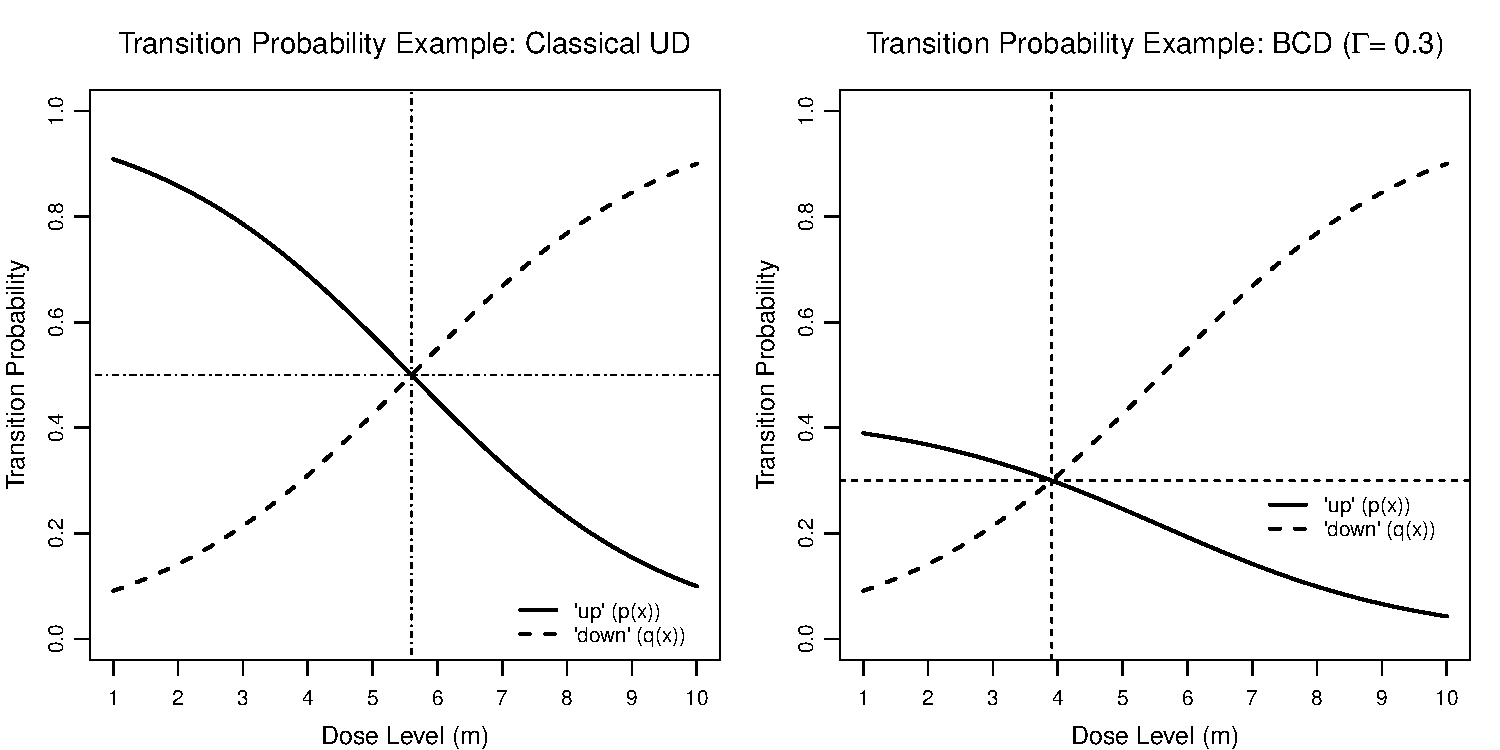
\includegraphics[scale=0.55]{pqfig}
\caption{The `up' and `down' transition probability functions $p(x)$ (solid line) and $q(x)$ (dashes), for classical UD (left) and BCD with $F^*=\Gamma=0.3$ (right), using hypothetical logistically-distributed toxicity threshold scenario and $M=10$ levels. The crosshairs denote $x=x^*$ and $y=F^*$.}\label{fig:pq}
\end{center}
\end{figure}

In dose-finding in general and in UD designs in particular, it is easy to focus on the central tendency and on asymptotic properties, and forget the magnitude of sampling variability that might be observed in practice. While UD designs do guarantee an $x^*$-centered random walk, it is still a random walk. Since most dose-finding applications use small samples, the relative magnitude of sampling variability is often rather substantial. In order to keep the reader cognizant of this variability, and to illustrate the concept of a random walk on $\mathcal{X}$, Figure~\ref{fig:traject} shows the experimental trajectories generated by three $n=30$ random draws from the same toxicity-threshold distribution, on an $M=8$ dose set, for each of the two designs described in Section~\ref{sec:tour}. The plots follow the graphical conventions common to dose-finding studies, with filled circles representing toxicities and empty ones non-toxicities. Balance points are denoted by dashed horizontal lines. The squares denote \emph{reversal points} in the experimental trajectories, whose properties are explored later.

We now describe a few first-order designs, called thus because they generate first-order Markov chains. For these chains, the probability of transiting to an adjacent dose in $\mathcal{X}$ depends upon the dose-allocation history, only through the current dose level and the current experimental outcome.

\chapter{A Tour Through First-Order Up--and--Down Designs}\label{sec:tour}
\section{The Classical Up--and--Down Rule}

The original (hereafter: ``classical'') UD design follows this rule: given $X_i=d_m$,
\begin{equation*}
X_{i+1}=
\begin{cases}
d_{m+1} &\textrm{if $Y_i=0$};\\
d_{m-1} &\textrm{if $Y_i=1$};\\
\end{cases}
\end{equation*}
for $m=2,\ldots,M-1$. In words, the experiment moves \emph{up} one level following a non-toxicity, and \emph{down} one level following a toxicity; hence the name \emph{up-and-down}. On the boundaries of $\mathcal{X}$, replace $d_0$ with $d_1$ whenever the former is mandated, and similarly replace $d_{M+1}$ with $d_M$ (i.e., the experiment stays on the boundary rather than venture outside it, which is impossible by design). Subsequently, boundary conditions are omitted since they always follow this basic adjustment.

The classical UD remains the most commonly used UD design. In the interior of $\mathcal{X}$ it leads to the following transition probabilities:

\begin{equation}
\begin{array}{rl}
p_{m,m+1}&=P\{Y_i=0|X_i=d_m\}=1-F(d_m);\\
p_{m,m-1}&=P\{Y_i=1|X_i=d_m\}=F(d_m).
\end{array}
\end{equation}
The balance point (\ref{eq:deftarget}) is the dose $x^*$ whose toxicity rate $F^*$ obeys
\begin{equation*}
1-F^*=F^*\ \longrightarrow \   F^*=0.5.
\end{equation*}
As expected from its symmetric transition rules, the classical UD design is best suited for estimating the median toxicity threshold.

\begin{figure}
\begin{center}
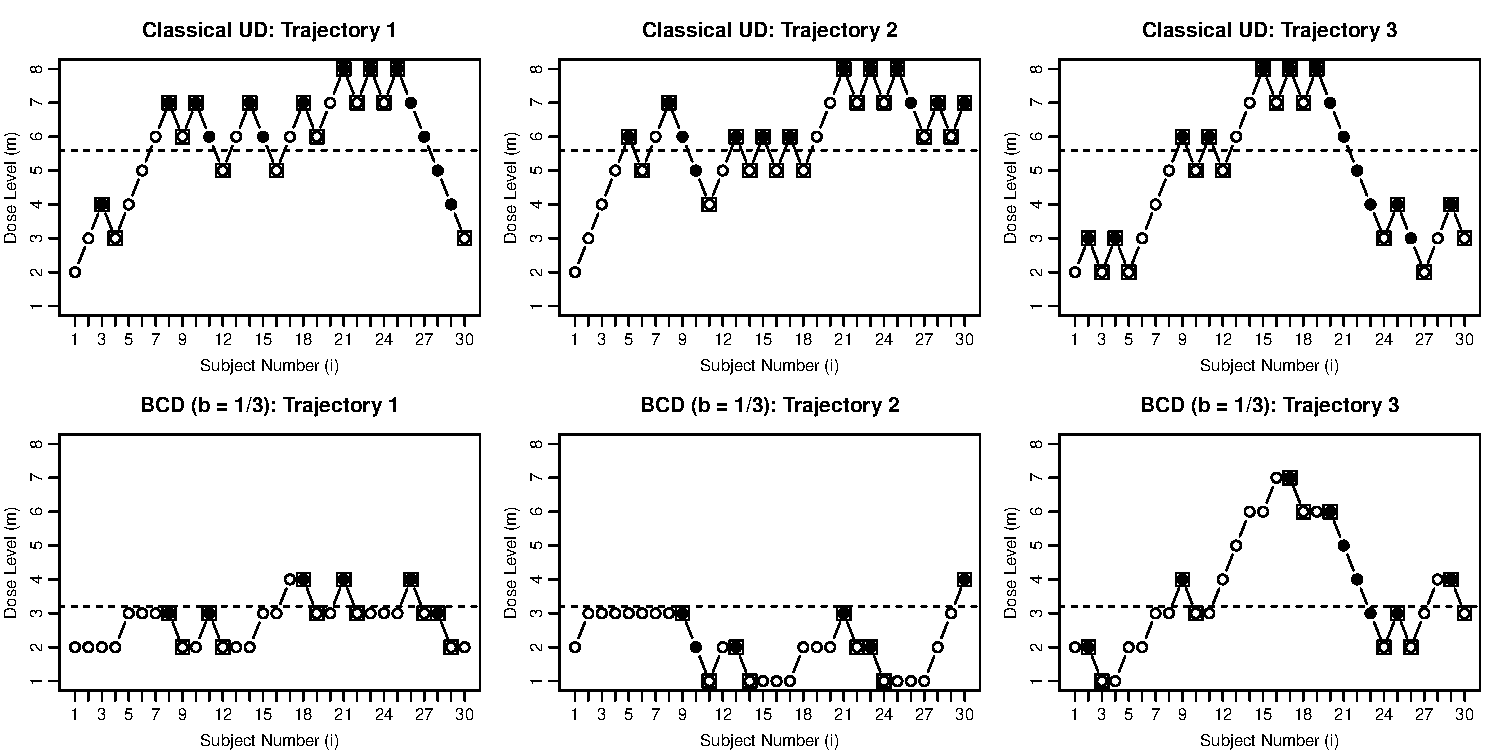
\includegraphics[scale=0.65]{Traject2}
\caption{Randomly generated ``experimental'' trajectories of classical UD for median estimation (top), and BCD with $b=1/3$ for estimating the 25th percentile (bottom), under a Gamma-distributed toxicity threshold density $f$, and $M=8$ levels. All runs begin at $X_1=d_2$. Toxicity responses are marked with filled circles, non-toxicities with empty circles. The balance point $x^*$ is marked by a horizontal dashed line. The squares denote \emph{reversal} points.}\label{fig:traject}
\end{center}
\end{figure}

\section{Biased Coin Up-and-Down Designs}

\subsection{Derman's Biased Coin Design}
\cite{Derm:Nonp:1957} was the first to develop an UD extension for non-median percentiles. His design requires a random toss of a metaphoric ``coin'', with $b=P\{\textrm{heads}\}\in[0.5,1]$. Given $X_i=d_m$,
\begin{equation*}
X_{i+1}=
\begin{cases}
d_{m+1} &\textrm{if $Y_i=0$, or}\\
d_{m+1} & \textrm{if $Y_i=1$ and `tails'; }\\
d_{m-1} &\textrm{if $Y_i=1$ and `heads'.}
\end{cases}
\end{equation*}
The balance point $x^*$ is given by
\begin{equation}\label{eq:dermanx*}
\begin{array}{rcl}
p(x^*)&=&q(x^*);\\
1-F\left(x^*\right)+(1-b)F\left(x^*\right) &=& bF\left(x^*\right);\\
F^*=F\left(x^*\right) &=& \frac{1}{2b}\in[0.5,1].
\end{array}
\end{equation}
%
For example, to produce a central tendency around the dose $F^{-1}(2/3)$, set $b=0.75$. When $b=1$, the balance point is the median, and indeed this value makes Derman's design identical to the classical UD design. A mirror-image version of the design (i.e, de-escalate after a toxicity and toss a `coin' after a non-toxicity) can be used to estimate percentiles below the median.

\subsection{Durham and Flournoy's  Biased Coin Design}\label{sec:bcd}

Derman's design has a practically unappealing property: if the coin points `tails', the experiment will move in the direction opposite to that indicated by the most recent response (i.e., the dose will escalate despite having just observed a toxic response). This is especially undesirable in clinical trials, where such transitions might actually halt the experiment due to safety concerns \citep[e.g.,][]{Neunsch08}. Not surprisingly, Phase~I researchers prefer designs that preclude such occurrences, which \cite{Cheung:coherent:05} called \emph{``incoherent''} dose transitions.\footnote{Not to be confused with the usage of ``coherence'' in Bayesian theory.}

\cite{Durh:Flou:rand:1994} suggested a design that uses a biased coin that centers the dose-allocation distribution around any percentile without ``incoherent'' transitions. Given $X_i=d_m$, the next dose allocation will be

\begin{equation}\label{eq:DF_BCD}
X_{i+1}=
\begin{cases}
d_{m+1} &\textrm{if $Y_i=0$ \& `heads'};\\
d_{m-1} &\textrm{if $Y_i=1$};\\
d_m &\textrm{if $Y_i=0$ \& `tails'}.\\
\end{cases}
\end{equation}

The `heads' probability $b$ can take any value in $[0,1]$. The balance point is given by
\begin{equation}\label{eq:bcdx*}
\begin{array}{rcl}
    b\left(1-F^*\right) &=& F^*\\
    F^* &=& \frac{b}{1+b}\in[0,0.5].
\end{array}
\end{equation}
%
Given a desired toxicity rate $\Gamma$, the BCD balance point can made identical to $F^{-1}(\Gamma)$ by setting the `heads' probability to $b=\Gamma/(1-\Gamma)$. For example, for $\Gamma=0.3$ (commonly used in Phase~I cancer trials) set $b=3/7$. Once again, setting $b=1$ makes this design identical to the classical UD, and inverting the rules produces above-median balance points. Hereafter, we refer to this design simply as the BCD.

The conditioning of dose escalation upon the outcome of a random draw in addition to a non-toxicity, keeps experimental trajectories at lower doses, on average, than the classical UD design does. In Figure~\ref{fig:traject} (bottom row), each BCD ``run'' with $b=1/3$ (i.e., $F^*=0.25$) uses exactly the same toxicity thresholds as the classical UD trajectory (i.e., $F^*=0.50$) shown immediately above it in the top row (all drawn randomly from a Gamma distribution). While the classical UD design runs escalate rather easily to the upper half of the $M=8$ dose range, the BCD runs are confined mostly to the bottom half.

\cite{Durh:Flou:rand:1994} also presented the \emph{reflected biased coin design} (RBCD) for estimating quantiles with toxicity rates greater than 0.05, as are typical for studies of efficacy rather than toxicity: Given $X_i=d_m$, the next dose allocation will be

\begin{equation}\label{eq:DF_RBCD}
X_{i+1}=
\begin{cases}
d_{m+1} &\textrm{if $Y_i=0$ };\\
d_{m-1} &\textrm{if $Y_i=1$ \& `heads'};\\
d_m &\textrm{if $Y_i=0$ \& `tails'}.\\
\end{cases}
\end{equation}

The `heads' probability $b$ again can take any value in $[0,1]$. So the balance point for the RBCD is given by
\begin{equation}\label{eq:rbcdx*}
\begin{array}{rcl}
    b\left(F^*\right) &=& 1-F^*\\
    F^* &=& \frac{1}{1+b}\in[0.5,1.0].
\end{array}
\end{equation}
%

\section{The Asymptotic Dose--Allocation Distribution}\label{sec:pi}

Because UD sequences of assigned doses $x_1,\ldots,x_n$ possess the properties of a Markov chain, as $n\to\infty$ the relative proportions of subjects assigned to each dose in $\mathcal{X}$ approach the \emph{asymptotic} or \emph{stationary allocation distribution} $\boldsymbol{\pi}=\left(\pi_1,\ldots,\pi_M\right)^{\prime};\ \ \sum_m \pi_m=1.$  If $\mathbf{P}$ is regular, then $\pi_m>0\ \forall m$. The distribution $\boldsymbol{\pi}$ can be found by solving the $M$ \emph{balance equations}, which is greatly simplified by the tri-diagonal structure of $\mathbf{P}$ for first-order UD designs (\ref{eq:genericPmat}):
%greatly simplifies the global balance equations. Splitting $\mathcal{X}$ into two groups by ``cutting'' it down the middle between any two adjacent dose levels $d_m,d_{m+1}$ without loss of generality, the balance equations between the two groups simplify to
\begin{equation}\label{eq:balance}
\pi_m=\pi_{m-1}p_{m-1,m}+\pi_mp_{mm}+\pi_{m+1}p_{m+1,m},\quad m=2,\ldots,M-1.
\end{equation}
The solution is a recursive formula for calculating $\boldsymbol{\pi}$ from the transition probabilities:
\begin{equation}\label{eq:balance_solution}
\pi_{m+1}=\lambda_m \pi_m,\ \ \ \lambda_m=\frac{p_{m,m+1}}{p_{m+1,m}},\ \  m=1,\ldots,M-1,
\end{equation}
where $\lambda_m$,  the \emph{adjacent-level ratio}, is the ratio between the single-step probabilities of escalating from $d_m$ and de-escalating to $d_{m}$. To ensure that $\sum_m \pi_m=1$, the base-level frequency $\pi_1$ is set by
\begin{equation*}
\pi_1^{-1}=1+\displaystyle\sum_{m=1}^{M-1}\displaystyle\prod_{j=1}^m\lambda_j.
\end{equation*}

\subsection{Calculating the Asymptotic Dose--Allocation Distribution for the Biased Coin
and Classical Up--and--Down Designs}

For the BCD, calculation of the adjacent-level ratio $\lambda_m$ is straightforward:
\begin{equation}\label{eq:BCDlambda}
\lambda_m=\frac{p_{m,m+1}}{p_{m+1,m}}=\frac{F^*}{\left(1-F^*\right)}\frac{\left(1-F(d_m)\right)}{F(d_{m+1})}.
\end{equation}
The same ratio is obtained for the RBCD.
 The numerator is monotone decreasing in $m$ while the denominator is increasing, and therefore, $\lambda_m$ as a whole is monotone decreasing. The doses for which $\{\lambda_m\}$ straddle unity bound the balance point $x^*$.

Interestingly, the classical UD presents a somewhat nonstandard asymptotic allocation distribution. Since $p_{mm}=0$ except on the boundaries, classical UD Markov chains are \emph{quasiperiodical}. For example, suppose the experiment begins at $d_5$, and $M=10$; then for subjects with an odd index $i$ the allocated dose level $m$ will be odd, and vice versa -- unless and until the trajectory hits upon a boundary and remains there for two consecutive subjects. If the design had no boundaries, then the chain would be purely periodical with a period of 2, yielding two non-communicating stationary distributions $\boldsymbol{\pi}^{(odd)},\boldsymbol{\pi}^{(even)}$. With finite $\mathcal{X}$, the classical UD design has a single $\boldsymbol{\pi}$ with the monotone decreasing adjacent-level ratio $\lambda_m=\left(1-F(d_m)\right)/F(d_{m+1})$.

\begin{figure}
\begin{center}
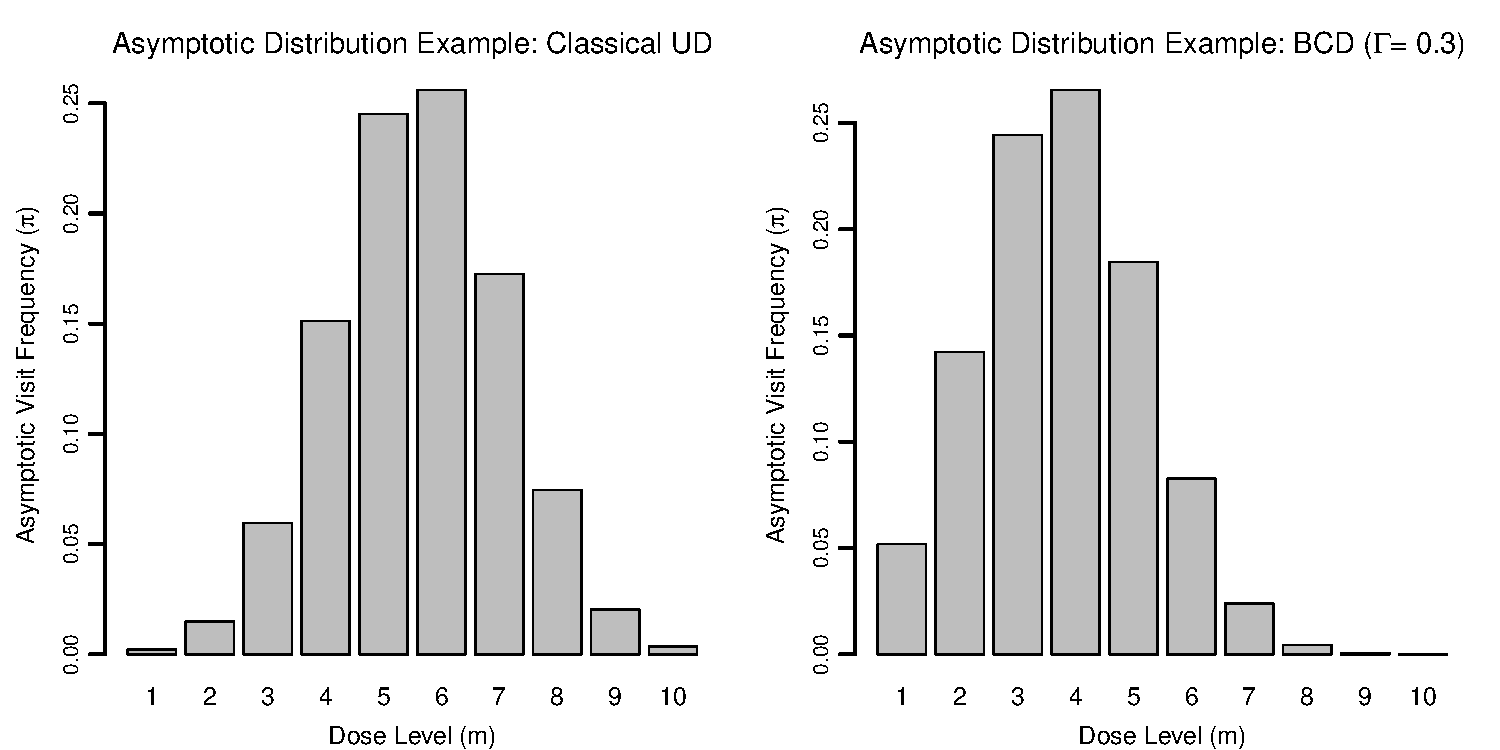
\includegraphics[scale=0.55]{pifig}
\caption{The asymptotic dose-allocation distribution $\boldsymbol{\pi}$ for the classical UD (left) and BCD with $\Gamma=0.3$ (right), using the same $\mathcal{X}$ and $F$ as in Figure~\ref{fig:pq}.}\label{fig:pi}
\end{center}
\end{figure}

\subsection{Unimodality of the Asymptotic Dose--Allocation Distribution and its Relationship to the Balance Point}\label{sec:modeloc}

 If $\lambda_m$ is monotone decreasing in $m$, as was just shown for the classical UD design and BCD, then it immediately follows that $\boldsymbol{\pi}$ is \emph{unimodal}:

\begin{itemize}
\item  If $\lambda_1\leq 1$ (or $\lambda_M\geq 1$), then $\pi_1\geq\pi_2\geq\cdots\geq\pi_M$ (or vice versa), and $\boldsymbol{\pi}$ has a single mode on the lower (upper) boundary.
\item If $\lambda_1\geq 1\geq\lambda_M$, then the $\pi_m$ initially increase as $m$ increases, then once $\lambda_m\leq 1$ they monotonically decrease -- thereby creating a single mode.
\end{itemize}

Unimodality of $\boldsymbol{\pi}$ is very useful if the mode's location is close to $x^*$ and if -- as stipulated earlier -- the design is chosen so that $F^*\approx\Gamma$ , because then the UD information collection rate about $F(x)$ eventually peaks around the percentile of interest (see e.g., Figure \ref{fig:pi}).\footnote{As long as $F(x)$ is strictly increasing, and transition probabilities are strictly monotone functions of $F(x)$ (as is the case for both classical UD and BCD), then scenarios when $\lambda_m=1$ will be all but nonexistent. If such a case does occur, the maximum value in $\boldsymbol{\pi}$ will be shared by two adjacent levels, called a \emph{modal set}, which together can be still seen as forming a single mode. In other words, qualitatively the design will still behave as do designs with a single-dose mode.} The following theorem guarantees this property, and is a cornerstone of UD design theory:
%
\begin{thm}\label{thm:mode} Consider an UD design generating a Markov chain, with an asymptotic allocation distribution $\boldsymbol{\pi}=\left(\pi_1,\ldots \pi_M\right)$ over $\mathcal{X}$, with $p(x)$ ($q(x)$) strictly monotone decreasing (increasing) in $x$, and a balance point $x^*$ as defined in (\ref{eq:deftarget}). If there exist two adjacent levels $d_{m^*}$ and $d_{m^*+1}$ such that $x^*\in\left[d_{m^*},d_{m^*+1}\right]$, then $\boldsymbol{\pi}$'s mode is either at $d_{m^*}$ or at $d_{m^*+1}$. Otherwise, the mode is on the boundary closest to $x^*$.
\end{thm}
%
\begin{proof} First, assume that $x^*\in\left[d_{m^*},d_{m^*+1}\right]$. Under the specified monotonicity conditions, the following inequalities always hold for any $2\leq m<M$:
%
\begin{equation}\label{eq:gammas1}
\lambda_{m-1}\ \ =\ \ \frac{p(x)\big |_{x=d_{m-1}}}{q(x)\big |_{x=d_m}}\ \ >\ \ \frac{p(x)\big |_{x=d_m}}{q(x)\big |_{x=d_{m}}}\ \ >\ \ \frac{p(x)\big |_{x=d_m}}{q(x)\big |_{x=d_{m+1}}}\ \ =\ \ \lambda_m\ .
\end{equation}
\noindent The ratio in the middle of this inequality is monotone decreasing in the dose $x$, and becomes exactly 1 at $x=x^*$. Therefore, for all $m<m^*$, $\lambda_m>1$ and for all $m>m^*$, $\lambda_m<1$. This means that the mode of $\boldsymbol{\pi}$ has to be at either $d_{m^*}$ or $d_{m^*+1}$.

\noindent On the lower boundary of $\mathcal{X}$, if $x^*<d_1$, then $\lambda_1=p_{12}/p_{21}<p\left(x^*\right)/q\left(x^*\right)=1$ and therefore the mode is at $d_1$. The upper-boundary case is analogous.\qed\end{proof}
%
Versions of Theorem~\ref{thm:mode} in varying degrees of generality, have appeared in the literature from \cite{Derm:Nonp:1957} onward. The formulation used above is adapted from \cite{Oron:Hoff:thek:2009}. In plain terms, the mode of $\boldsymbol{\pi}$ is guaranteed to be at one of the two dose levels straddling the balance point $x^*$.

Whether the asymptotic mode is in fact on the single closest level to $x^*$ depends upon the design, and upon how ``closest'' is defined. Defining ``closeness'' on the toxicity-frequency ($F$) scale, rather than on the dose ($x$) scale, is generally more useful. For example, the following property was proven for the classical UD:
%
\begin{thm}\label{thm:modesud}
\citep{Oron:Hoff:thek:2009}
For the classical UD design, $\boldsymbol{\pi}$'s mode is at the level whose toxicity rate is closest to $0.5$.
\end{thm}
\begin{proof} Let $x^*=F^{-1}(0.5)\in [d_{m^*},d_{m^*+1}]$. Write $F\left(d_{m^*}\right)=0.5-\Delta p_1$ and $F\left(d_{m^*+1}\right)=0.5+\Delta p_2$, where $\Delta p_1\geq 0$ and $\Delta p_2\geq 0$. Then the adjacent-level ratio (\ref{eq:balance_solution}) at level $m^*$ can be written as
\begin{equation}\label{eq:sudmode}
\lambda_{m^*}=\frac{p_{m^*,m^*+1}}{p_{m^*+1,m^*}}=\frac{0.5+\Delta p_1}{0.5+\Delta p_2}.
\end{equation}
\noindent Because $\lambda_{m^*}\geq 1$ if and only if $\Delta p_1\geq\Delta p_2$, the result immediately follows from this inequality.\qed
\end{proof}
%
For the BCD, the mode is not necessarily the dose closest to the target. Let $x^*=F^{-1}(\Gamma),\ \Gamma<0.5$, and cast the BCD adjacent-level ratio (\ref{eq:BCDlambda}) into a form analogous to (\ref{eq:sudmode}), to obtain
\begin{equation*}
\lambda_{m^*}=\frac{p_{m^*,m^*+1}}{p_{m^*+1,m^*}}=\frac{\Gamma\left(1-\Gamma+\Delta p_1\right)}{(1-\Gamma)\left(\Gamma+\Delta p_2\right)}.
\end{equation*}
%
\noindent This adjacent-level ratio is greater than 1 if and only if $\Delta p_1/\Delta p_2>(1-\Gamma)/\Gamma$. For example, if $\Gamma=1/4$ and $x^*\in\left[d_2,d_3\right]$, then the asymptotic mode will be at $d_2$ unless $F\left(d_3\right)$ is 3 times closer to $1/4$ than $F\left(d_2\right)$. This means that the BCD's dose-allocation behavior is somewhat more conservative (i.e., less amenable to dose escalation) than indicated by its nominal target toxicity rate.

\subsection{Sharpness of the Asymptotic Dose--Allocation Distribution}

The unimodality of $\boldsymbol{\pi}$ helps concentrate information collection around $x^*$. It is also of practical interest to know how steeply $\boldsymbol{\pi}$ decreases to either side of its mode, in order to know the degree of this concentration and the frequency of excursions away from $x^*$. Assume without loss of generality, that the mode is at a single interior level $d_{m^*}$. Due to monotonicity conditions, we know that $\lambda_{m^*-1}>1$ and $\lambda_{m^*}<1$. If the adjacent-level ratios remained constant at these values on either side of the mode, then the rate of decrease in $\boldsymbol{\pi}$ values away from the mode would be geometric -- the discrete analogue of exponentially-decreasing tails. However, due to their monotonicity, the $\lambda$'s become \emph{more} extreme as one moves away from the mode. Hence, the drop in asymptotic allocation frequencies away from $\boldsymbol{\pi}$'s mode is faster than geometric for UD designs.


\section{Characteristics of the Durham--Flournoy Biased Coin Design When the Dose--Toxicity Function is Logistic}\label{sec:logistic}
\section{The Asymptotic Dose--Allocation Distribution}
\cite{Durh:Flou:rand:1994} obtained a valuable result (shown in Theorem~\ref{thm:discnormal} below) regarding the form of the BCD's $\boldsymbol{\pi}$ and the steepness of this decrease away from the mode. This result requires the following definition:
\begin{defn}
Let $Z$ be a random variable that is defined on a set of discrete
real valued points $\mathcal{X}$.  Let $\tilde{\Phi}(z)$ denote $P\{Z=z\}$.  Then $Z$ is said to have a \emph{Discrete Normal Distribution} if
\begin{equation*}
\tilde{\Phi}(z_j)=\frac{e^{-\frac{1}{2}z_j^2}}{\sum_{i=1}^Me^{-\frac{1}{2}z_i^2}},\,\,\,z_j\in\mathcal{X}.
\end{equation*}
\end{defn}
\begin{thm}\label{thm:discnormal}
Assume that subjects' toxicity thresholds are logistically distributed, with $$1-F(x)=(1+\exp(\mu+\tau x))^{-1,}\ \ \tau>0,$$ and that the doses are equally spaced: $\mathcal{X}=\{d_1<d_1+\Delta,d_1+2\Delta<\cdots<d_1+(M-1)\Delta\}.$ Then the BCD and the RBC have the same asymptotic allocation distribution, which is a mixture of two discrete normal distributions over $\mathcal{X}$,  and  the mixing parameter is the target toxicity rate $\Gamma$, that is,
%
\begin{equation}\label{eq:discnormal}
\pi_m=(1-\Gamma)\tilde{\Phi}\left(\frac{d_m-(x^*-0.5\Delta)}{\sqrt{\Delta/\tau}}\right)+
\Gamma\tilde{\Phi}\left(\frac{d_m-(x^*+0.5\Delta)}{\sqrt{\Delta/\tau}}\right),\ \ d_m\in\mathcal{X}.
\end{equation}
\end{thm}
%
See section \ref{sec:logitproofs} and \cite{Durh:Flou:rand:1994} for the proof.

The modes of the two discrete normal distributions are separated by one dose spacing unit $\Delta$, so they have considerable overlap. If $\Gamma=0.5$, i.e., the design is the classical UD procedure, the mixture is equally weighted and, as shown in more generality in Theorem~\ref{thm:modesud}, the asymptotic mode will be on the dose whose toxicity rate is closest to $0.5$. Conversely, as $\Gamma\to 0$ the first component will dominate, shifting the asymptotic mode as far as $\Delta/2$ downwards.

Despite the specific parametric assumptions on $F$,  (\ref{eq:discnormal}) provides a useful guideline about the stationary frequency of BCD excursions, because many common response function models are very similar except on the extreme tails, and because (as will be shown later) several common UD designs produce $\boldsymbol{\pi}$s at least as sharp as those of the BCD.

Under the assumptions of Theorem~\ref{thm:discnormal}, roughly 97.5\% of the allocations will be within $x^*\pm 2\sqrt{\Delta/\tau}$.  This approximation can be used to choose $\Delta$ so as to control for highly toxic events, given approximate prior knowledge of the dispersion parameter $\sigma$ \citep{Durh:Flou:Rose:rand:1997}.

The following theorem asserts that the first and second components of (\ref{eq:discnormal}) are the asymptotic allocation distribution for subjects with non-toxic and toxic responses, respectively.  The proof is in section~\ref{sec:logitproofs}.
\begin{thm}\label{thm:logitpi|y}
Allocated doses according to BCD or RBCD under the assumptions of Theorem~\ref{eq:discnormal}, then
\begin{equation}
\pi_m=(1-\Gamma)P(X_n=d_m|Y_n=0)+\Gamma P(X_n=d_m|Y_n=1).
\end{equation}
\end{thm}
 %


\subsection{Illustrations}
{\bf Assaf: insert redo of allocation histograms separately, with side by side bars, for toxicities and non-toxicity - this would require redo of prior histogram assuming logistics F.  Otherwise, have overall figure and side by side bars side by side for comparison.  Let's talk about this. it would be nice to have enough levels that the normality shape appears.}



\subsection{Proofs of Theorems~\ref{thm:discnormal} and \ref{thm:logitpi|y}}\label{sec:logitproofs}
\subsubsection{Proof of Theorem~\ref{thm:discnormal}}
The BCD and RBCD have identical adjacent-level ratios~(\ref{eq:BCDlambda}) which, given logistic toxicity rates, are
\begin{align*}
\lambda_m&=\frac{p_{m,m+1}}{p_{m+1,m}}
=\frac{\Gamma }{(1-\Gamma)}\frac{(1-F_m)}{F_{m+1}}
\\&=exp\left(\mu+\tau x^*\right)\frac{1}{1+exp\left(\mu+\tau x_m\right)}\, 
\frac{1+exp\left(\mu+\tau x_{m+1}\right)}{exp\left(\mu+\tau x_{m+1}\right)}, \ m=1,\ldots,M-1.
\end{align*} 
Noting that $x_m=(m-1)\Delta$, the stationary dose-allocation probabilities can be written as
\begin{align*}\label{eq:BCDpilogit}
\pi_{m}=\prod_{j=1}^m \lambda_j &= \lambda_1 \frac{exp(k (\mu+\tau x^*))}{1+exp\left(\mu+\tau x_1\right)}\,
\frac{1+exp\left(\mu+\tau x_m\right)}{exp\left((m-1)(\mu+\tau x_)+(m-1)m \Delta \tau/2\right)}\\
&= \lambda_1 \frac{1+exp\left(\mu+\tau x_m\right)}{1+exp\left(\mu+\tau x_1\right)}\,
exp\left(-\frac{-2\left(x_m-x_1\right)\left(x^*-x_1-0.5\Delta\right)\left(x_m-x_1\right)^2}{2\tau^2}
\right).
\end{align*}
Define $\overline{x^*}=x^*+0.5\Delta$ and $\underline{x^*}=x^*-0.5\Delta$; complete the square and simplify (\ref{eq:BCDpilogit}) by changing variables; namely, let 
$\overline{z}_m=(x_m-x^*)/\sqrt{\Delta/\tau}$ and $\underline{z}_m=(x_m-x^*)/\sqrt{\Delta/\tau}$.  Now (\ref{eq:BCDpilogit}) can be written as
\begin{equation}
\pi_{m}= \frac{\lambda_1}{1+exp\left(\mu+\tau x_1\right)}\,
\left(exp\left(-\frac{\underline{z}_m^2}{2}+\frac{\underline{x^*}^2}{2\Delta/\tau}\right)
+exp\left(\mu-\frac{\overline{z}_m^2}{2}+\frac{\overline{x^*}^2}{2\Delta/\tau}\right)\right).
\end{equation}
Because the total allocation proportions sum to one,, we have from () that
\begin{align}\label{eq:lamda-1logit}
\lambda_1^{-1}= & \frac{1}{1+exp\left(\mu+\tau x_1\right)}\,
\left(exp\left(\frac{\underline{x^*}^2}{2\Delta/\tau}\right)\sum_{j=1}^M exp\left(-\frac{\underline{z}_m^2}{2}\right)\right.\\
&\, \,\left. +exp(\mu)\, \left(exp\left(\frac{\overline{x^*}^2}{2\Delta/\tau}\right)
\sum_{j=1}^M exp\left(\frac{\overline{z}_m^2}{2}\right)\right)\right).
\end{align}
Since the two sums differ only by the first and last terms, $\mathcal{X}$ can be arranged so that these terms are small, making the two sums approximately equal {\bf(work this into assumptions above)}.  Assuming this is the case, and using (\ref{eq:lambda-1logit}), the result follows.

\subsubsection{Proof of Theorem~\ref{thm:logitpi|y}}
The marginal probability of no toxicity can be written as
\begin{align}
P(Y_n=0)&=\sum_m P(Y_n=0|X_n=d_m)P(X_n=d_m)\\
&=\frac{1}{1+exp\left(\mu+\tau x^*\right)}
\end{align}


Substituting () directly into () yields
\begin{equation}
\pi_m=\tilde{\Phi}(\underline{z_j})\frac{1+exp\left(\mu+\tau x_m\right)}{1+exp\left(\mu+\tau x^*\right)}
=\tilde{\Phi}(\underline{z_j})\frac{P(Y_n=0|X_n=x^*)}{P(Y_n=0|X_n=x_m)}.
\end{equation}
$\tilde{\Phi}(\underline{z_j})$

\section{Up--and--Down Convergence}

\subsection{Convergence of the Dose~Allocation Process to Stationary Behavior}\label{sec:geom}

The presentation of asymptotic UD properties has thus far sidestepped an important practical aspect. Dose-finding experiments are by their nature small-to-medium-sample affairs ($n<100$, and more often than not $n<30$), so asymptotic behavior would generally not dominate the magnitude of observed variability -- as we reminded the reader at the close of Section~\ref{sec:intro}. So why bother about asymptotic behavior at all? Indeed, in recent years dose-finding analyses have rarely examined asymptotic behavior, relying almost exclusively upon numerical simulations instead.

As \cite{oron:azri:hoff:dose:2011} argue, this recent view is misguided. An obvious practical reason is that simulations are, generally speaking, haphazard rather than systematic samples from the space of all relevant dose-toxicity scenarios, and are therefore prone to misuse and abuse -- as anyone who has read enough simulation-based dose-finding articles can attest. But an even stronger,  \emph{conceptual} reason is that all sequential dose-finding designs rely upon some mechanism for concentrating dose allocations near the target. How good is the mechanism?

A straightforward test is to allow the design to run indefinitely, and characterize its behavior. A design with a good concentrating mechanism must demonstrate reasonably desirable behavior as $n\to\infty$. Conversely, if desirable asymptotic behavior \emph{cannot} be guaranteed, or if the type of convergence or conditions for convergence make asymptotic behavior all-but-impossible for dose-finding applications, then the design should probably not be trusted even for small-to-medium $n$. Hence the importance of asymptotics (discussed above) and convergence, to which we turn our attention now.

With sequential procedures such as UD designs, the term ``convergence'' carries many different meanings. Results have been published about the convergence of UD dose-allocation frequencies \citep{Durh:Flou:up-a:1995,Durh:Flou:Mont:up-a:1995}, and about the convergence of observed toxicity rates \citep{Flou:Durh:Rose:toxi:1995,oron:azri:hoff:dose:2011}. A third type of convergence is the convergence of \emph{the dose-allocation process itself}, which in the case of UD designs is convergence to stationary sampling from $\boldsymbol{\pi}$.

For Markov chains, convergence of the dose-allocation process to stationary behavior erases, or ``mixes'', the arbitrary initial conditions. A deterministically chosen starting dose can be represented by an allocation distribution $\boldsymbol{\rho}$ which is 0 everywhere and 1 at $d_m=x_1$. In the case of a completely random starting point, $\boldsymbol{\rho}$ has a discrete-uniform distribution over $\mathcal{X}$. The allocation distribution after the first subject can be written in matrix form as $\boldsymbol{\rho}^{'}\mathbf{P}$ (see (\ref{eq:genericPmat})). The probability distribution of the $n+1$-th assignment, given the starting conditions only, is $\boldsymbol{\rho}^{'}\mathbf{P}^n$ \cite[cf.,][]{Diac:Stro:geom:1991}. All rows of $\mathbf{P}^n$ become arbitrarily close to $\boldsymbol{\pi}$ as $n\to\infty$, meaning that from some $n$ onwards the marginal allocation distribution of subsequent doses becomes essentially stationary, and independent of the initial conditions $\boldsymbol{\rho}$. Specifically,
\begin{equation}\label{eq:diac}
\max_m\left|{\mathbf{P}}^n_{m}-\boldsymbol{\pi}^\prime\right|\propto\beta_2^n,\ \ m=1,\ldots M,
\end{equation}
\noindent where $|\cdot| $ denotes Euclidean distance; ${\mathbf{P}}^n_{m}$ is the  $m$-th row of $\mathbf{P}^n$; and $\beta_2$ is the eigenvalue of $\mathbf{P}$ with the second-largest absolute value.\footnote{
The largest absolute eigenvalue of $\mathbf{P}$ is 1, associated with the stationary behavior itself.} Since it is known that $\left|\beta_2\right|<1$, the allocation-distribution convergence rate is geometric in $n$ --  far faster than the usual root-$n$ rate of the laws of large numbers and many other processes.

The practical implication of geometric convergence is that while individual UD allocation sequences might vary (see Fig.~\ref{fig:traject}), the impact of initial conditions is erased at a rate fast enough to bear fruit even during a small-sample experiment. \cite{Oron:Hoff:thek:2009} translated the geometric rate to terms relevant for experimentalists. They progressed the allocation distribution from the initial conditions $X_1=d_1$, and observed how many subjects it would take the expectation $\mathrm{E}{(n)}[X]$ of the allocation distribution at subject $n$,  to reach $99\%$ of the way from $d_1$ to the stationary mean $\mathrm{E}{(\infty)}[X]=\sum_m \pi_m d_m$. Several UD designs targeting $\Gamma=0.3$ were examined under several dose-toxicity scenarios each. With $M=5$ levels, it took 10-20 subjects to arrive $99\%$ of the way to $E_{(\infty)}[X]$, and with $M=10$ about twice as long.

\subsection{A Law of Large Numbers for the Empirical Allocation Frequencies}
Let $W_j(n)$ denote the proportion of subjects allocated to dose $d_j$.  For UD rules with regular transition probability matrix $\mathbf P$, independent of the starting dose, $$P\left(|W_j(n)-\pi_j|\longrightarrow 0\right). $$

\subsection{A Central Limit Theorem for the Empirical Allocation Frequencies}\label{sec:asymvar}

The convergence of \emph{empirical} dose allocations at the individual dose levels is also of great practical importance. For example, the quality of the isotonic regression estimator of the target percentile $F^{-1}(\Gamma)$ (see below and Section~\ref{sec:est}), depends upon this distribution being clustered around the target. We know that if $F^*\approx\Gamma$, then asymptotically this is the case. But is this true for real-life sample sizes?

%\citep{ford,Ford:Tors:Wu:use:1992}).  Such allocations are incompatible with UD designs which concentrate allocations around $x^*$.   We know that if $F^*\approx\Gamma$, then asymptotically the UD design concentrates data collection in the vicinity of $\Gamma$, which will be relatively efficient for regression estimates of $F^{-1}(\Gamma)$ which ideally would have all the allocations at the doses that straddle $x^*$.

Let $\mathbf{W}(n)=\left(W_1(n),\ldots ,W_M(n)\right)$ denote the empirical allocation distribution, i.e., the proportion of subjects allocated to each level when $n$ subjects have been allocated in total. Then for UD designs, the asymptotic distribution of $\mathbf{W}$ is determined by the central limit theorem (CLT) for regular Markov chains:
%
\begin{equation}\label{eq:CLT}
\sqrt{n}\left(\left(W_1(n),\ldots, W_m(n)\right)-\boldsymbol{\pi}^\prime\right)\,
\stackrel{\mathcal{L}}\longrightarrow
\ \mathcal{N}\left(0,diag\left[\sigma_1^2(\mathbf{P})
,\ldots ,\sigma_M^2(\mathbf{P})\right] \right),
\end{equation}
as $n\rightarrow \infty$ where $\sigma^2_j=2\pi_jz_{jj}-\pi_j-\pi_n^2$ and $z_{jj}$ is the $j$th diagonal element of  $\mathbf{Z}=(\mathbf{I}-\mathbf{P}+\boldsymbol{\Pi})^{-1}$.

\cite{Frec:1938} used the so called \textit{fundamental
matrix} $\mathbf{Z}$ to avoid the use of
eigenvalues in expressing the limiting variance of a Markov chain.
 \citep[see also Chapter 11, pg 464]{Grin:Snel:Intr:1997}.

 Since software is now readily available for calculating eigenvalues, we also provide
 an
expression for $\sigma_k^2(\mathbf{P})$ from
 \cite{Bort:Giov:Upan:2005}  which is a special case of a representation given by
 \cite{Pesk:opti:1973}:
\begin{equation}\label{eq:MCrxvar}
\sigma_k^2(\mathbf{P})=w_k^2\sum_{i=1}^K\frac{1+\lambda_{[i]}}{1-\lambda_{[i]}}
\left(v_{k[i]}\right)^2,\,\,\,i,k=1,\ldots,K,
\end{equation}
where $\lambda_{[i]}$ denotes the $i$th largest eigenvalue of {$\mathbf
P$} in absolute value and $v_{k[i]}$ denotes the $k$th component of
the corresponding normalized left eigenvector of ${\mathbf{P}}$.


%
The rate of convergence is of order $\mathrm{O}\left(1/\sqrt{n}\right)$ -- the usual CLT rate. This is one reason why the empirical mode of allocated doses, examined in some recent studies as an estimator for $F^{-1}(\Gamma)$, performs rather poorly in that role despite its asymptotic consistency \citep{Giov:Pint:Pint:prop:1998}. At $n=30$ or even $60$, the variability in allocated proportions is too high to reliably equate the empirical mode with the stationary mode.

Note: from a practical perspective, choosing a design with smaller asymptotic variances $\left(\sigma_1^2(\mathbf{P}),\ldots,\sigma_M^2(\mathbf{P})\right)$ is equivalent to increasing the scaling constant of the convergence rate, i.e., accelerating the convergence. Both will help $\mathbf{W}(n)$ achieve a pre-specified precision threshold with fewer subjects. However, the overall root-$n$ convergence rate cannot be changed, and it is far slower than the convergence of the dose-allocation process itself to stationary behavior.

\section{Estimating a Quantile of the Dose--Toxicity Function}

More often than not, estimation of UD experiments has been approached inconsistently by both applied and methodological researchers. Many researchers use outdated and questionable estimators of $F^{-1}(\Gamma)$, just because these estimators happen to be prevalent in their field. Many method developers illogically produce  UD estimates  in the same way as estimates from an entirely different class of dose-finding designs \cite[e.g.,][]{Zack:stag:2009}. To help alleviate the confusion, Section~\ref{sec:est} is dedicated mostly to UD estimation. Right now, a brief description is provided for two  estimators of $F^{-1}(\Gamma)$: the one most commonly used for the classical UD design, and a more recent estimator considered as standard for the BCD and recommended for all UD designs.

\subsection{Reversal--Averaging Estimators}

The most common classical UD estimator for the median-toxicity dose uses \emph{reversal points} -- those subjects in the experiment whose toxicity outcome is different from the outcome of the immediately previous subject:
%
\begin{equation}\label{eq:reversal}
\mathcal{R}=\left\{i:\ Y_i\neq Y_{i-1},\ i=2,\ldots ,n\right\},
\end{equation}
where $Y_i$ is subject $i$'s binary toxicity outcome. Reversal points are surrounded by squares in Figure~\ref{fig:traject}. The reversal estimator of $F^{-1}(\Gamma)$ is a simple average of the doses at which reversals are observed:
\begin{equation}\label{eq:reversav}
\overline{X}^{\mathrm{(rev.)}}=\frac{\sum_iX_iI\left[i\in\mathcal{R}\right]}{\sum_iI\left[i\in\mathcal{R}\right]},
\end{equation}
\noindent where $I[\cdot]$ is the indicator function. Sometimes the first few reversals are excluded in order to mitigate the starting-dose bias. Using reversals rather than all assigned doses is done mostly for historical reasons \citep{Weth:Chen:Vasu:est:1966}. As explained more fully in Section~\ref{sec:est}, we recommend the discontinuing  the averaging of only reversal doses.

\subsection{Isotonic--Regression Based Estimators}

\cite{Styl:Flou:dose:2002} adapted isotonic regression \citep{BBBB:order:1972} for estimating $F^{-1}(\Gamma)$ following UD experiments. For dose-toxicity applications, isotonic regression begins by calculating the empirical toxicity frequencies at each dose,
%
\begin{equation}\label{eq:fhat}
\hat{F}_m=\frac{\sum_{i=1}^n Y_iI\left[X_i=d_m\right]}{\sum_{i=1}^n I\left[X_i=d_m\right]},\ m=1,\ldots,M.
\end{equation}
%
The somewhat awkward formulation in (\ref{eq:fhat}) is equivalent to simply tabulating how many observations were made at each dose, and what proportion of these are toxicities. For example, if 4 subjects have thus far been given dose $d_m$ with 2 toxicities, then $\hat{F}_m=0.5$.

In the case of a monotonicity violation among the $\{\hat{F}_m\}$, isotonic regression recursively replaces adjacent pairs of violating values by their weighted average, until all violations disappear and the resulting estimate conforms to the assumption of an increasing dose-toxicity relationship. Stylianou and Flournoy's estimate for $F$ in $[d_1,d_M]$ linearly interpolates between the isotonic-regression pointwise results. The dose where $\hat{F}$ crosses the horizontal line $y=\Gamma$ becomes the UD point estimate of $F^{-1}(\Gamma)$. This estimator is a special case of \emph{regression estimators}: estimators that fit some curve \ $y=\hat{G}(x)$ through the points $\left\{\left(d_m,\hat{F}_m\right)\right\}$.  Dose-response plots and isotonic regression estimators for the six simulated runs of Figure~\ref{fig:traject} are shown in Figure~\ref{fig:isot}, along with a minor modification called ``centered isotonic regression'' \citep[Section~3.3]{Oron07}.
%
\begin{figure}
\begin{center}
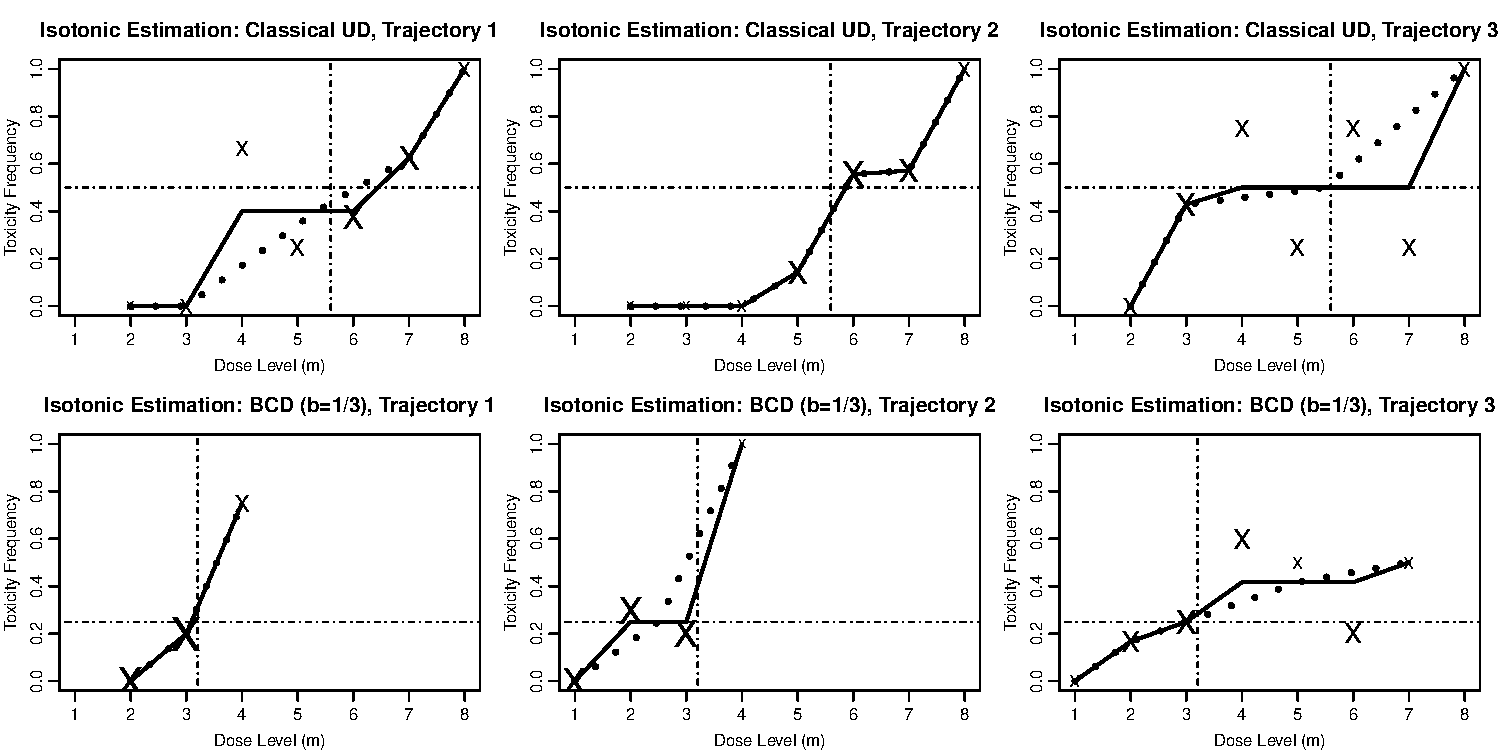
\includegraphics[scale=0.65]{isot}
\caption{Dose-response plots display cumulative toxicity rates $\mathbf{\hat{F}}$
for each of the randomly-generated scenarios of Figure~\ref{fig:traject} and for both the classical UD design ($\Gamma=0.50$, top) and the BCD with $b=1/3$ ($\Gamma=0.25$, bottom): 'x' symbols mark the proportion of subjects receiving dose $d_m$; isotonic regression estimates are given by the solid lines; and centered-isotonic regression estimates are given by the dotted lines.  The respective point estimates of $F^{-1}(\Gamma)$ are the $x$ values where the solid lines cross the dash-dot horizonal $y=\Gamma$ lines. The true quantile is marked with a dash-dot vertical line.}\label{fig:isot}
\end{center}
\end{figure}


\chapter{Exact Statistics for First Order Up--and--Down Designs}

\section{Exact Moments of the Dose Allocation Frequencies}

\subsection{Expected Dose Allocation Frequencies}\label{sec:trialfrequencies}
After $n$ subjects have been put on trial, the proportion of subjects treated at each dose $k=1,\ldots,K$ is $W_k(n)=n^{-1}\sum_{m=1}^n\textrm{I}(X_m=d_k)$.
%
The set of first moments, $\{\mathrm{E}[W_k(n)]\}_{k=1}^K$, gives the expected allocation distribution; second moments permit the construction of confidence intervals of the allocation frequencies at each dose.  Functions of the moments, such that the expected number of subjects treated at a high dose level, are discussed later.

For notational simplicity, the subscript $\mathbf{p}$ in $P_{\mathbf{p}}(\cdot)$,
$\mathrm{E}_{\mathbf{p}}(\cdot)$, etc., indicates that the probabilities and
expectations are taken with respect to the initial probability distribution $\mathbf{p}$ of
$X_1$; in the special case in which the initial dose is not
random and $\mathbf{p}$ is degenerate, the subscript $i$ indicates
that the probabilities are conditional on a fixed initial dose
$X_1=d_i$.  The expected relative dose-allocation frequencies are
\begin{align}\label{eq:E_i(W_k(n))}
\mathrm{E}_i\left[W_k(n)\right]
&=\frac{1}{n}\mathrm{E}\left[\sum_{m=1}^n\textrm{I}[X(m)=x_k]|X_1=d_i\right]\nonumber \\
&=\frac{1}{n}\sum_{m=1}^np_{ik}(m)=\frac{1}{n}\left(\delta_{ik}+
\sum_{m=2}^np_{ik}(m)\right),\quad k=1,\ldots, K,
\end{align}
where $\textrm{I}[\cdot]$ denotes the indicator function. Let $\tilde{\mathbf{w}}(n)$ denote the $K\times K$ dimensional matrix
with $i$th row vector $\mathrm{E}_i[\mathbf{w}(n)]$.  Then
$\mathrm{E}_{\mathbf{p}}[\mathbf{w}(n)]
=\sum_{i=1}^K\mathrm{E}_i[W_k(n)]p_i(1)$, or
%
\begin{equation}\label{eq:E_p(W(n))}
\mathrm{E}_{\mathbf{p}}[\mathbf{w}(n)]
=\bf{p}(1)\tilde{\mathbf{w}}(n)
\end{equation}
when $X_1$ is random with probability distribution $\mathbf{p}(1)$.

When the initial distribution is the asymptotic distribution,
(\ref{eq:E_p(W(n))}) becomes $\mathrm{E}_{\boldsymbol{\pi}}[\mathbf{w}(n)]=\boldsymbol{\Pi}$, where
$\mathbf{\Pi}$ is the $K\times K$ matrix whose rows are all $\boldsymbol{\pi}$.

\subsection{A Recursion Algorithm for Updating Expected Allocation Frequencies after Making Observations on a New Subject}
By the Markov property of the allocation rules,
(\ref{eq:E_i(W_k(n))}) can be expressed as a recursion for serial
updating after each subject:
\begin{align*}
n\mathrm{E}_i\left[W_k(n)\right]&=p_{ik}(1)+\sum_{m=2}^n\sum_{l=1}^Kp_{il}p_{lk}(m-1)\\
&=\delta_{ik}+\sum_{l=1}^Kp_{il}\sum_{m=2}^np_{lk}(m-1)\\
&=\delta_{ik}+\sum_{l=1}^Kp_{il}\sum_{m=1}^np_{lk}(m)\\
&=\delta_{ik}+(n-1)\sum_{l=1}^Kp_{il}\mathrm{E}_i\left[W_{k}(n-1)\right],
\quad k=1,\ldots,K.
\end{align*}
Expressing this recursion in matrix notation is useful for
computing with software such as MATLAB:
\begin{align*}
n\tilde{\mathbf{w}}(n)&=\bf{I}+\mathbf{P}\tilde{\mathbf{w}}(n-2)
=\bf{I}+\mathbf{P}+\mathbf{P}^2+\cdots
+\mathbf{P}^{n-2}+\mathbf{P}^{n-1},
\end{align*}
where $\mathbf{I}$ is the identity matrix.

\subsection{The Variance of a Dose Allocation Frequency}\label{sec:allocationvariances}
We show in section (\ref{sec:allocationcov}) that  when $X_1$ is
fixed at $d_i$, the variance of the dose-allocation frequency at level $k$, after the $n$th allocation,   is given by
\begin{align*}
n^2\ \textrm{Var}_i\left[W_k(n)\right]
=\sum_{s=1}^np_{kk}(t)\left(\delta_{kk}-p_{ik}(t)\right)
+
2\sum_{s>t} p_{kk}(s-t)p_{ik}(t)-p_{ik}(s)p_{ik}(t),\\
%
\ n\ge 1,\ \ k,l=1,\ldots,K.
\end{align*}
Then for any subject $n\ge 1$, when the first dose $X_1$ is allocated with
probability $\mathbf{p}(1)$,
\begin{flushleft}
$n^2\textrm{Var}_{\mathbf{p}}\left[W_k(n)\right]$
\end{flushleft}
\begin{equation*}
=\sum_{s=1}^n \displaystyle\sum_{i=1}^Kp_{lk}(t)\left(\delta_{lk}-p_{ik}(t)\right)p_i(1)
+2\sum_{s>t}^n p_{kk}(s-t)p_{ik}(t)-\displaystyle\sum_{i=1}^Kp_{ik}(s)p_{ik}(t)p_i(1).
\end{equation*}

\subsection{First Allocation and Mean Recurrence Times}
Given a subject is allocated to dose  $d_k$, the recurrence time  is the number of subjects allocated before another subject is allocated to $d_k$.  We know the asymptotic allocation distribution is unimodal.  But these times help gauge how often excursions into the tails of the distribution are likely to occur.   Also, if one starts allocations at the lowest (highest) dose, the mean recurrence times indicate how long it will take the allocation process to reach, say, the middle or the far edge of the dose space.

Suppose a subject has just been allocated to dose $d_k$, and let  $m_{kl}$ denote the mean number of subjects allocated until dose $d_k$ is allocated again.
Then $$m_{kl}=\frac{z_{jj}-z_{ij}}{\pi_j},\, k\ne l.$$
Suppose again that a subject has just been allocated to dose $d_k$, and let $r_k$ denote the mean number of subjects is takes for the dose allocation process to return to dose $d_k$.  Then $$r_k=\frac{1}{\pi_k}. $$
{See Chapter 11, Theorems 11.15 and 11.6}\cite{Grin:Snel:Intr:1997}.

{bf give example of analyzing the effect of starting at lowest dose, perhaps for different densities of dose levels and/or different slopes of F}

\subsection{ A Graphical Tool for Determining when {\em n} is Large Enough for Asymptotic Approximations}
{\bf This section needs to be rewritten:}

Recall the fundamental matrix for regular Markov chains:
 $\mathbf{Z}=\left(z_{ik}\right)=\left({\mathbf{I}}+\left({\mathbf{P}}
 -\boldsymbol{\Pi}\right)\right)^{-1}$.
  We show below that
when starting from any particular level, say $i$,
$$n\mathrm{E}_{\mathbf{p}}\left[W_k(n)\right]-nw_k \ \ \stackrel{\textrm{as } n
\rightarrow \infty}\longrightarrow\ \ z_{ik}-w_k. $$
A plot of $n\mathrm{E}_{\mathbf{p}}\left[W_k(n)-w_k\right]$ by $n$ is will asymptote at
the constant $z_{ik}-w_k$. When $n\mathrm{E}_{\mathbf{p}}\left[W_k(n)-w_k\right]$  gets close to its asymptote, large sample approximations will
provide satisfactory statistics for UD designs.

 Recall that $\boldsymbol{\Pi}=\boldsymbol{\pi}'\bf{1}$, where $\bf{1}=(1\cdots 1)$,
$\boldsymbol{\Pi}^n=\boldsymbol{\Pi}$ for all $n$ and
$\boldsymbol{P}^n-\boldsymbol{\Pi} \stackrel{\textrm{as } n \rightarrow \infty}\longrightarrow 0$,
 it follows  \citep[see][pg 22]{Keme:Snel:1960}) that
\begin{align}\label{fundamental_matrix}
\lim_{n \rightarrow \infty} n(\tilde{\mathbf{w}}(n)-\boldsymbol{\Pi})&=\lim_{n
\rightarrow \infty}\left({\mathbf{I}}+\sum_{m=1}^n\left(\mathbf{P}^m-\mathbf{\Pi}\right)\right) \nonumber =\left(\mathbf{I}+\left(\mathbf{P}-\boldsymbol{\Pi}\right)\right)^{-1}.
\end{align}
It follows from (\ref{fundamental_matrix}), that when any
particular starting level is chosen, say $i$,
$n\mathrm{E}{\mathbf{p}}\left[W_k(n)\right]-nw_k\rightarrow z_{ik}-w_k$ as $n
\rightarrow \infty$.  Thus for large $n$,
\begin{equation}\label{lrgenfreqappox}
\mathrm{E}{\mathbf{p}}\left[W_k(n)\right] \approx\frac{z_{ik}+nw_k}{n}.
\end{equation}
To calculate (\ref{lrgenfreqappox}), use the definition of a
particular up-and-down design to calculate the transition
probabilities $\{p_{ij}\}$; then use (\ref{eq:balance}) to
calculate the asymptotic treatment distribution $\mathbf{w}$ which
are the rows of $\boldsymbol{\Pi}$. $\mathbf{Z}$ can then be calculated using a
standard matrix inversion routine.

Furthermore, it follows from (\ref{eq:E_p(W(n))}) and
(\ref{fundamental_matrix}) that for any initial distribution $\mathbf{p}(1)$,
\begin{align}
\lim_{n \rightarrow \infty}\mathrm{E}{\mathbf{p}}\, n\left[\mathbf{{\tilde
W}}(n)-\boldsymbol{\Pi}\right]&=\lim_{n \rightarrow
\infty}np(1)\sum_{m=1}{n}\left(\mathbf{P}^m-\boldsymbol{\Pi}\right) \nonumber\\
&=\mathbf{p}(1)\left(\mathbf{Z}-\mathbf{\Pi}\right)
=\mathbf{p}(1)\mathbf{Z}-\boldsymbol{\Pi}.
\end{align}

By (\ref{fundamental_matrix}) for large $n$, the difference
between $\mathrm{E}_{\mathbf{p}}n\left[W_k(n)-nw_k\right]$ is approximately equal to
the constant $z_{ik}-w_k$. Thus a plot of
$\mathrm{E}_{\mathbf{p}}\left[nW_k(n)-nw_k\right]$ by $n$ approaching this constant can
serve as a tool for deciding when large sample approximations will
be satisfactory.
%
 %
\subsection{Covariances between Dose--Allocation Frequencies at Different Dose Levels}\label{sec:allocationcov}
The covariances between
dose-allocation frequencies are sums  of the covariances between
dose allocations for each subject; and the covariances between dose allocations for each subject can be calculated from
the transition probabilities. After $n$ subjects, when $X_1$ was
fixed at $d_i$, the covariances between dose-allocation frequencies at levels $k,l=1,\ldots,K$ for $n\ge 1$  are
\begin{equation*}
Cov_i\left[W_k(n),W_l(n)\right]
=\frac{1}{n^2}\sum_{s=1}^n\sum_{t=1}^nCov_i\left[\textrm{I}\left[X(s)=x_k\right],
\textrm{I}\left[X(t)=x_l\right]\right],
\end{equation*}
where the covariance between an allocation to dose $x_k$ for subject $s$ and an allocation to dose
$x_l$ for subject $t$ is
%
\begin{flushleft}
$Cov_i\left[\textrm{I}\left[X(s)=x_k\right],\textrm{I}\left[X(t)=x_l\right]\right]$\\
\end{flushleft}
\begin{equation*}
=
\begin{cases}
p_{lk}(s-t)p_{il}(t)-p_{ik}(s)p_{il}(t) &\textrm{if $s>t$},\\
p_{kl}(t-s)p_{ik}(s)-p_{ik}(s)p_{il}(t) &\textrm{if $s<t$},\\
p_{lk}(t)\left(\delta_{lk}-p_{il}(t)\right) &\textrm{if $s=t$}.\\
\end{cases}
\end{equation*}
Then for any subject $n\ge 1$, when the first dose $X_1$ is allocated with
probability $\mathbf{p}(1)$,
\begin{equation*}
Cov_{\mathbf{p}}\left[W_k(n),W_l(n)\right]
=\frac{1}{n^2}\sum_{s=1}^n\sum_{t=1}^nCov_{\mathbf{p}}
\left[\textrm{I}\left[X(s)=x_k\right],\textrm{I}\left[X(t)=x_l\right]\right],
\end{equation*}
where the covariance between an allocation to dose $x_k$ for subject $s$ and
an allocation to dose $x_l$ for subject $l$ is
\begin{flushleft}
$Cov_{\mathbf{p}}\left[\textrm{I}\left[X(s)=x_k\right],\textrm{I}\left[X(t)=x_l\right]\right]$
\end{flushleft}
\begin{equation*}
=
\begin{cases}
p_{lk}(s-t)p_{il}(t)-\displaystyle\sum_{i=1}^Kp_{ik}(s)p_{il}(t)p_L(1) &\textrm{if $s>t$},\\
p_{kl}(t-s)p_{ik}(s)-\displaystyle\sum_{i=1}^Kp_{ik}(s)p_{il}(t)p_L(1) &\textrm{if $s<t$},\\
\displaystyle\sum_{i=1}^Kp_{lk}(t)\left(\delta_{lk}-p_{il}(t)\right)p_L(1) &\textrm{if $s=t$}.
\end{cases}
\end{equation*}
To evaluate large sample properties of these covariances it is
helpful to define a $K\times K$ matrix $\vec{\textrm{C}}$ with elements
\begin{equation*}\label{c_kl}
c_{kl}=\lim_{n\rightarrow\infty}n\textrm{Cov}_{\mathbf{W}}\left[W_k(n),W_l(n)\right].
\end{equation*}
Since
$\lim_{n\rightarrow\infty}\mathrm{E}[{\mathbf{p}}(\cdot)]=\lim_{n\rightarrow\infty}
\mathrm{E}[{\mathbf{W}}(\cdot)]$
for all initial treatment distributions ${\mathbf{p}(1)}$, for $n$
sufficiently large it is sufficient to consider $\mathbf{X}(1)$ to be
random with asymptotic probability distribution $\mathbf{W}$.  Thus
$c_{lk}$ provides a large sample approximation to
$n\textrm{Cov}_{\mathbf{p}}\left[W_k(n),W_l(n)\right]$ that is
independent of $\mathbf{p}(1)$.

Let $\mathbf{D}_W=diag\left(w_1,w_2,\ldots,w_K\right)$.  Expressing
$c_{kl}$ in terms of the asymptotic probabilities and the
fundamental matrix (\ref{fundamental_matrix}) makes them easily
computable:
\begin{equation*}
\mathbf{C}=\mathbf{D}_w-\mathbf{w}'\mathbf{w}
+\mathbf{D}_{\mathbf{w}}(\mathbf{Z}-\mathbf{I})
+(\mathbf{Z}'-\mathbf{I})\mathbf{D}_{\mathbf{w}}.
\end{equation*}
A proof of this relationship can be found in Kemeny and Snell
~\cite{Keme:Snel:1960}.  So a tractable large sample
approximation to $\textrm{Cov}_{\mathbf{W}}\left[W_k(n),W_l(n)\right]$ that is
independent of $\mathbf{p}(0)$ is suggested by (\ref{c_kl}), namely,
$$\textrm{Cov}_{\mathbf{W}}\left[W_k(n),W_l(n)\right]\approx {c_{kl}}/n.$$


Durham, Flournoy and Montazer-Haghighi \cite{Durh:Flou:Mont:up-a:1993} showed that the
increment in the covariance between treatment frequencies is
approximately constant for large $n$:
\begin{equation}
n^2\left(\textrm{Cov}_{\mathbf{W}}\left[W_k(n+1),W_l(n+1)\right]
-\textrm{Cov}_{\mathbf{W}}\left[W_k(n),W_l(n)\right]\right)
\rightarrow c_{kl} \textrm{ as $n \rightarrow \infty$}.
\end{equation}
This greatly simplifies the required recursive computation for
large $n$.  It also provides a tool for determining when the large
sample approximation in (\ref{c_kl}) is suitable in that the
number of trials required can be read off from where a plot of the
increment versus $n$ approaches a constant.

\section{Moments of the Empirical Toxicity Frequencies}

\subsection{First and Second Moments of a Single Toxic Response}
As said before, conditional on allocation to dose $x_k$, the probability of a toxic response is $P_i(Y_n=1|d_x)=F(d_k)$ for all $n$ independent of the starting dose $d_i$; and the conditional variance of $Y_n$ is
$\textrm{Var}_i\left[Y_n|d_x\right]=F(d_k)\left(1-F(d_k)\right)$.
Unconditionally a toxic response from  the $n$th subject  is a Bernoulli random variable with
$$P_i(Y_n=1)=\sum_{k=1}^K P_i(Y_n=1|X_n=d_k)p_{ik}=\sum_{k=1}^KF(d_k)p_{ik}(n)\,\, \stackrel{n\rightarrow\infty}\longrightarrow \,\,
\sum_{k=1}^KF(d_k)\pi_k,$$
given the initial subject was allocated to dose $d_i$.  The variance of $Y_n$ is
\begin{align*}
\textrm{Var}_i\left[Y_n\right]&=P_i(Y_n=1)\ P_i(Y_n=0)
=\left(\sum_{k=1}^KF(d_k)p_{ik}(n)\right)\left(1-\sum_{k=1}^KF(d_k)p_{ik}(n)\right)\\
&=\sum_{k=1}^KF(d_k)p_{ik}(n)-\sum_{k=1}^K\left(F(d_k)p_{ik}(n)\right)^2\\
&\stackrel{n\rightarrow\infty}\longrightarrow \,\,
\sum_{k=1}^KF(d_k)\pi_k-\sum_{k=1}^K\left(F(d_k)\pi_k\right)^2.
\end{align*}
The covariance between a toxic response from two subjects $m$ and $n$ who were both allocated to dose $d_k$ is
\begin{align*}
\textrm{Cov}\left[Y_m,Y_n\right]
&=\textrm{E}\left[Y_m\ Y_n\right]-\textrm{E}\left[Y_m\right]\textrm{E}\left[ Y_n\right]\\
&=P\left[Y_m=1, Y_n=1\right]-P\left[Y_m=1\right]P\left[Y_n=1\right]\\
&=\sum_{k=1}^K(F(d_k))^2\textrm{Cov}_i\left[\textrm{I}[X_m=d_k,X_n=d_k]\right]-\sum_{k=1}^K(F(d_k))^2p_{ik}(m)p_{ik}(n)
\end{align*}

\subsection{Exact First and Second Moments of the Total Number of Toxicities}
The total number of toxicities up to and including the $n$th trial is the sum of dependent Bernoulli random variables.  Let $R(n)=\sum_{m=1}^nY(m)$ denote the total number of toxicities after $n$ trials.
Theorem
\begin{align*}
&\textrm{(i)}\  \mathrm{E}_{\mathbf{p}}[R(n)]=\sum_{k=1}^K \left(F(d_k) \sum_{m=1}^n p_{ik}\right), \ \ k=1,\ldots,K;\\
&\textrm{(ii)}\  \lim_{n\rightarrow\infty} \frac{1}{n} \mathrm{E}_{\mathbf{p}}[R(n)]=   \sum_{k=1}^K F(d_k) \boldsymbol{\pi}_{\mathbf{p}} \\
%&\textrm{(iii)}\  \textrm{Var}_i[R(n)]=\sum_{m=1}^n
% \left(\sum_{k=1}^K F(d_k) p_{ik}-\sum_{k=1}^K \sum_{l=1}^K F(d_k)F(d_l)  p_{ik}p_{il}
% \right)+
% \sum_{m=1}^n  \sum_{s=1}^n  \left(\sum_{k=1}^K  \left(\sum_{l=1}^K
% F(d_k)  F(d_l)\left[g_{kl}(m+1-s)-p_{il}(m+1) \right]p_{ik}(s)+F(d_i)P(d_i)
%  p_{ik}-\sum_{k=1}^K \sum_{l=1}^K F(d_k)F(d_l)  p_{ik}p_{il};
 %    \\
%&\textrm{(iv)}\  \lim_{n\rightarrow infty}n^{-1}\textrm{Var}_i[R(n)]
%=\sum_{k=1}^K F(d_k) \pi_k - \left(\sum_{k=1}^K  F(d_k)  \pi_k\right)^2
%+2 \sum_{k=1}^K \sum_{l=1}^K F(d_k)F(d_l) \pi_k
%\left(g_{k,k-1}z_{k-1,l}+g_{kk}z_{kl}+g_{k,k+1}z_{k+1,l}-\pi_l
%\right),  \\
\end{align*}
where $z_{kl}=\delta_{kl}+\sum_{s=1}^{infty}\left[p_{kl}-\pi_l\right]$, $z_{kl}$ is the $(k,l)$th element from the \textit{fundamental matrix for regular Markov chains}  \citep{see, for example}{pg. 75, 77}{keme:snel:1960}), and $\delta_{kl}$ is Kroneker's delta.

%%%%%%%%%%%%%%%%%%%%%%%%%%%%%%% SECTION 2 STARTS HERE
\section{Proofs of Theorems ....}


\chapter{Higher-Order Up--and--Down Designs and Other Extensions}\label{sec:extens}

Via first-order designs, we have now completed a brief tour of the main UD design properties and estimation approaches. The first-order BCD (with the classical UD design as a special case) is simple and intuitive, and allows for the estimation of any percentile. However, there are cases when neither the classical UD design nor BCD are adequate, such as when
\begin{itemize}
\item Subjects are treated in cohorts rather than individually, in order to save time and resources;
\item In some applications, such as oncology, researchers are reluctant to use randomization in a toxicity study, even for selecting between two adjacent doses (as required for the BCD);
\item Other UD designs may yield better estimation efficiency.
\end{itemize}
This section surveys additional, somewhat more sophisticated UD designs that are either in common use or have been studied in some detail. When relevant, they are compared with the BCD and to each other. The section ends with a description of an innovative UD design for dose-finding in which the target dose involves joint toxicity and efficacy probabilities.

\section{Group Up--and--Down Designs}\label{sec:gud}

Group up--and--down rules were first introduced in the 1960's for median estimation, by \cite{Weth:Sequ:1963} and \cite{Tsut:asym:1967,Tsut:rand:1967}, and more recently studied in greater depth by \cite{Gezm:Flou:Grou:2006}, \cite{Ivan:esca:2006} and \cite{Bald:Bort:Giov:2008} for the estimation of any percentile. Subjects are treated in cohorts of a fixed size $s$. Let $l$ and $u$ be two integers such that $0\le l< u\le s$. With a group UD design, $Y_i$ is the number of toxic responses in the $i$-th cohort, rather than a binary outcome. Given that the $i$-th cohort is treated at $X_i=d_m$ on the interior of $\mathcal{X}$, the $i+1$-th cohort is assigned to
%
\begin{equation*}
X_{i+1}=
\begin{cases}
d_{m+1} &\textrm{if $Y_i\le l$ };\\
d_{m-1} &\textrm{if $Y_i\ge u$};\\
d_m &\textrm{if $l<Y_i<u$ }.
\end{cases}
\end{equation*}
%
Conditional upon $X_i$ and $F(x)$, $Y_i$ has a Binomial distribution with parameters $s$ and $F(d_m)$, with the `up' and `down' probabilities being the Binomial distribution's tails, and the `stay' probability its center (it is zero if $u=l+1$). This design rule is abbreviated as GUD$_{(s,l,u)}$.

Nominally, a GUD is an $s$-order design, since the $s$ most recent observations are needed to determine the next allocation. However, with cohorts viewed as single entities (with each entity containing $s$ subjects), the group UD generates a first-order Markov chain having a tri-diagonal TPM as in (\ref{eq:genericPmat}). In this \emph{condensed form}, it is straightforward to show that the Durham-Flournoy monotonicity conditions on $p(x)$ and $q(x)$ are met, and therefore, Theorem~\ref{thm:mode} holds and $\boldsymbol{\pi}$ is unimodal.   Unlike the classical UD design and the BCD, except for special cases GUD balance points can be calculated only numerically, by finding the dose $x^*$ with toxicity rate $F^*$ such that
%
\begin{equation}\label{eq:group_balance}
\sum_{r=u}^s
\left(\begin{array}{c}
s\\
r\\
\end{array}\right) \left(F^*\right)^r(1-F^*)^{s-r}=
\sum_{t=0}^{l}
\left(\begin{array}{c}
s\\
t\\
\end{array}\right) \left(F^*\right)^t(1-F^*)^{s-t}.
\end{equation}
%
Any numerical root-finding algorithm can be used to solve for $F^*$ in (\ref{eq:group_balance}). \cite{Gezm:Flou:Grou:2006} and \cite{Ivan:Flou:Chun:Cumu:2007} present tables with $(s,l,u)$ combinations, and the corresponding values of $F^*$ satisfying (\ref{eq:group_balance}). For example, GUD designs that might be useful for $\Gamma=0.3$ include the following combinations:

\begin{center}
\begin{small}
\begin{tabular}{lcccccccccccc}
\toprule
$s$ & 2 & 3 & 4 & & \multicolumn{2}{c}{5} &  &   \multicolumn{4}{c}{6} \\
\midrule
$(l,u)$ & (0,1)& (0,2)& (0,2)& & (0,3)& (1,2) & &  (0,3)& (1,2) &  (0,4)& (1,3) \\
$F^*$ & 0.293 &  0.347 & 0.267 & & 0.302 & 0.314  & & 0.253 & 0.264 & 0.326 & 0.341\\
\bottomrule
\end{tabular}
\end{small}
\end{center}

Notable special cases of group UD designs, whose $F^*$ can be calculated by hand, are symmetric ones ($u+l=s$) for which $x^*$ is the median (the classical UD design again is a special case of this family, namely GUD$_{(1,0,1)}$). In addition, the family GUD$_{(k,0,1)}$ is related to the design we describe next.

\section{The $k$--in--a--row (``Geometric'') Design}\label{sec:kr}
{\bf Expand this section a lot; put proof in a subsection at the end.}

The design called here the ``$k$--in--a--row design'' is presented in some detail, due to its widespread use in sensory studies  \citep{Treu:Mini:1995}, and to a now-resolved controversy regarding its properties.  The rule, whose development and introduction to sensory studies date back to Wetherill's work in the 1960s  \citep{Weth:Sequ:1963,Weth:Levi:Sequ:1966}, is extremely simple:
%
\begin{equation}\label{eq:krule}
 X_{i+1}=
 \begin{cases}
d_{m+1} &\textrm{ if $Y_{i-k+1}=\cdots=Y_i=0$}, \textrm{ all observed at $d_m$};\\
d_{m-1} &\textrm{ if $Y_i=1$}; \\
d_m &\textrm{otherwise},
 \end{cases}
\end{equation}
\noindent where $k\geq 1$ is an integer constant. In words, under this rule every dose escalation requires $k$ consecutive non-toxicities at the current level, while de-escalation only requires a single toxicity. Using straightforward reasoning, Wetherill concluded that this design's balance point at dose $x^*$ is given by
%
\begin{equation}\label{eq:krtarget}
 F^*=F\left(x^*\right)=1-\left(\frac {1}{2}\right)^{1/k}.
\end{equation}
%
\noindent The $k=1$ case is simply the classical UD design, but $k=2,3,4$ would be associated with $F^*\approx 0.293,0.206$ and $0.159$, respectively.\footnote{The method used in sensory studies is actually the mirror-image of (\ref{eq:krule}), with $k$ successive responses required for a de-escalation and only one non-response for escalation, yielding $F^*\approx 0.707,0.794,0.841,\ldots$.}

While Wetherill correctly identified $F^*$, the characterization of $k$--in--a--row's overall Markov chain behavior was provided only a generation later by \cite{Gezm:Geom:1996}, and completed by \cite{Oron:Hoff:thek:2009}. Recent work also gave the design the following names: first ``geometric UD design'' (for reasons that will be apparent soon) and then \emph{``$k$--in--a--row} '' design \citep{Ivan:Mont:Moha:Durh:impr:2003}, the name used here. Meanwhile, in sensory studies, where it is most commonly used, the design is known as ``forced-choice fixed-staircase methods'' \citep{Treu:Mini:1995}; but this name is used for related non-Markovian designs as well.

The $k$--in--a--row design generates a $k$-th order Markov chain because knowledge of the last $k$ responses might be needed. Like any $k$-order chain, it can be represented as a first-order chain with $Mk$ states, useful for writing out a transition probability matrix (TPM).\footnote{It should be noted that for the highest level $d_M$ internal states are redundant: no escalation is possible and therefore dose-transition behavior is identical and depends only on the most recent outcome. So the most concise representation of a $k$--in--a--row TPM would have $(M-1)k+1$ states. However, for symmetry and aesthetics we use $Mk$ states.} Equivalently,  it can be modeled as a Markov chain with $M$ levels, each having $k$ \emph{``internal states''} labeled $0$ to $k-1$ \citep{Oron:Hoff:thek:2009,Weiss:Aspe:1994}. The internal state serves as a counter of the number of immediately recent consecutive non-toxicities observed at level $m$. This description is closer to the physical dose-allocation process, because subjects at different internal states of the same level $m$ are all assigned the same dose $d_m$. Either way, the TPM is $Mk\times Mk$. Equation (\ref{eq:kPmat}) shows the expanded $k$--in--a--row TPM with $k=2$ and $M=6$, using the abbreviations $F_m=F\left(d_m\right),\bar{F}_m=1-F_m, m=1,\ldots,M$; dose levels are labeled.
%
\begin{equation}\label{eq:kPmat}
\mathbf{P}=\left[\begin{array}{p{1cm}cccccccccccc}
& \multicolumn{2}{c}{\emph{$m$=1}} & \multicolumn{2}{c}{\emph{$m$=2}}& \multicolumn{2}{c}{\emph{$m$=3}}& \multicolumn{2}{c}{\emph{$m$=4}}& \multicolumn{2}{c}{\emph{$m$=5}}& \multicolumn{2}{c}{\emph{$m$=6}} \\
  \multirow{2}{*}{\emph{$m$=1}} &  F_1 &\bar{F}_1 &0 &0 &0 &0 &0 &0 &0 &0 &0 & 0\\
   &  F_1 &0         &\bar{F}_1 &0 &0 &0 &0 &0 &0 &0 &0& 0\\
  \multirow{2}{*}{\emph{$m$=2}} &  F_2 &0 &0 &\bar{F}_2 &0 &0 &0 &0 &0 &0 &0& 0\\
 &   F_2 &0 &0 &0 &\bar{F}_2  &0 &0 &0 &0 &0 &0& 0\\
  \multirow{2}{*}{\emph{$m$=3}} &  0    &0 &F_3 &0 &0   &\bar{F}_3 &0 &0 &0 &0 &0& 0\\
  &  0    &0 &F_3 &0 &0   &0 &\bar{F}_3 &0 &0 &0 &0& 0\\
  \multirow{2}{*}{\emph{$m$=4}} &  0    &0 &0   &0 &F_4 &0 & 0&\bar{F}_4 &0 &0 &0 &0\\
  &  0    &0 &0   &0 &F_4 &0 &0      & 0   &\bar{F}_4 &0 &0 &0\\
  \multirow{2}{*}{\emph{$m$=5}} &  0    &0 &0   &0 &0   &0 &F_5    & 0   &0 &\bar{F}_5 &0 &0\\
  &  0    &0 &0   &0 &0   &0 &F_5    & 0   &0 &0 &\bar{F}_5 &0\\
 \multirow{2}{*}{\emph{$m$=6}} &   0    &0 &0   &0 &0   &0 &0         &0 &F_6 &0 & 0&\bar{F}_6\\
  &  0    &0 &0   &0 &0   &0 &0         &0 &F_6 & 0 &\bar{F}_6 & 0\\
\end{array}\right]
\end{equation}
The matrix is regular, assuring that there is an asymptotic distribution $\boldsymbol{\pi}^{\textrm{(states)}}$, with positive values for all $Mk$ states. This is not the asymptotic \emph{dose-allocation} distribution $\boldsymbol{\pi}$, since it counts separately different internal states of the same level $m$. The latter can be found by summing $\boldsymbol{\pi}^{\textrm{(states)}}$ over the internal states of each level.

\cite{Gezm:Geom:1996} found  $\boldsymbol{\pi}^{\textrm{(states)}}$ by noting that non-base ($>0$) internal states can only be accessed from the internal state immediately below in the same level. The balance equation for such states is, therefore,
%
\begin{equation}\label{eq:kinternal}
\pi^{\textrm{(states)}}_{m(j)}=\left(1-F_m\right)\pi^{\textrm{(states)}}_{m(j-1)},\ \ j=1,\ldots,k-1,
\end{equation}
\noindent where $m(j)$ denotes the internal state $j$ within dose level $m$. This is the formula of a decreasing geometric sequence with a quotient of $\left(1-F_m\right)$, hence the name Gezmu suggested for the design (``geometric UD design'').

Now, the balance equation between $d_m$ and $d_{m+1}$ is
%
\begin{equation}\label{eq:kexternal}
\pi^{\textrm{(states)}}_{m(k-1)}\left(1-F_m\right)=\pi_{m+1}F_{m+1},
\end{equation}
%
\noindent In words, `up' transitions are possible only from the top internal state, while `down' transitions are mandated upon any toxicity regardless of internal state. After applying standard geometric-series formulae to express $\pi^{\textrm{(states)}}_{m(k-1)}$ as a function of $\pi_m$ , one obtains the stationary adjacent-level ratio of the dose-allocation distribution $\boldsymbol{\pi}$:
%
\begin{equation}\label{eq:krgamma}
\lambda_m=\frac{F_m\left(1-F_m\right)^{k}}{F_{m+1}\left[1-\left(1-F_m\right)^{k}\right]}.
\end{equation}
%
This ratio is monotone decreasing in $m$, conforming to the Durham-Flournoy conditions
(see Section~\ref{sec:balpoint}). The $k$--in--a--row balance point can now be calculated; indeed, it is the one found by Wetherill~(\ref{eq:krtarget}). It is also identical to the balance point of GUD$_{(k,0,1)}$. The same unimodality and mode-location properties with respect to $x^*$ shown for $\boldsymbol{\pi}$ of the classical UD design and the BCD, hold for $k$--in--a--row as well \citep{Oron:Hoff:thek:2009}.\footnote{The derivation of (\ref{eq:krgamma}) assumes stationarity. For finite $n$, the marginal transition probabilities are very cumbersome to calculate; it is for the $k$--in--a--row design that the $n\to\infty$ limit terminology is needed in Definition~\ref{def:pxqx}.}

\section{Biased Coin Design Extensions}

The versatile framework of the BCD lends itself to further extensions.

\subsection{A Generalized Biased Coin Design}
Taking advantage of the flexibility in constructing biased coin designs, \cite{Bort:Giov:Upan:2005} examined a generalized first-order approach in order to study their properties. Let there be two coins having $\Pr\left\{\textrm{heads}\right\}$ equal to $b_1$ and $b_2$. Then
\begin{equation}\label{eq:BortotCombo}
X_{i+1}=
\begin{cases}
d_{m+1} &\textrm{if $Y_i=0$ and coin 1 yields heads};\\
d_{m-1} &\textrm{if $Y_i=1$ and coin 2 yields heads};\\
d_{m} &\textrm{if $Y_i=0$ and coin 1 yields tails}\\
        & \textrm{or $Y_i=1$ and coin 2 yields tails.}
\end{cases}
\end{equation}
\noindent The balance point maintains
\begin{equation*}
F^*b_2=\left(1-F^*\right)b_1;\ \ F^*=b_1/(b_1+b_2).
\end{equation*}
\noindent Setting $b_2=1$ yields Durham and Flournoy's BCD. A family of generalized BCDs for the same $\Gamma$ can be created by setting $$\frac{b_2}{b_1}=\frac{1-\Gamma}{\Gamma},\ b_2\in [0,1],$$ so it can be indexed by a single `coin-toss' parameter. Although all members of the family share the same balance point, they differ in other properties, as described below.

\subsection{Integrated Parallel Biased Coin Design Sequences}
\cite{Flou:aran:1998} proposed the use of an urn model to integrate parallel BCD runs, helping shorten an experiment's duration. This strategy is also useful when clinical trials are performed at different locations.

\section{A Second Order Biased Coin Design}
\cite{Bort:Giov:Upan:2005} also developed a second-order BCD, again using two coins. Given $X_i=d_m$,
%
\begin{equation*}
X_{i+1}=
\begin{cases}
d_{m+1} &\textrm{if $Y_i=0$, $Y_{i-1}=0$ and coin 1 yields heads}\\
        &\textrm{or $Y_i=0$, $Y_{i-1}=1$ and coin 2 yields heads}\\
d_{m-1} &\textrm{if $Y_i=1$}\\
d_m &\textrm{otherwise.}
\end{cases}
\end{equation*}
%
Bortot and Giovagnoli derived $\boldsymbol{\pi}$, and showed that it is unimodal by the Durham--Flournoy conditions (see Sec.~\ref{sec:balpoint}) and if $(1-\Gamma )b_1+\Gamma b_2=\Gamma /(1-\Gamma )$. However, their simulations indicate only a modest estimation performance improvement over the first-order BCD.

\subsection{A Generalized Group Up--and--Down Design}
\cite{Bald:Bort:Giov:2008} generalized the group UD design for any user-specified toxicity rate $\Gamma$ by adding a biased coin to the dose allocation procedure.
\chapter{Comparing Up--and--Down Designs}

With several UD variants to choose from for estimating a given quantile, some ways to compare UD designs are needed. An obvious comparison criterion is estimation performance -- e.g., mean square error (MSE) of the quantile estimates. Since estimates at the various dose levels are dependent, in general this practical metric can only be gauged via simulation studies. A more didactic approach that can often save simulation time, is to consider individual properties, and find \emph{theoretical} relationships between designs for these properties. Some properties suggested and examined by researchers are
%
\begin{itemize}
\item Convergence rates of the dose-allocation process and of empirical dose-allocation frequencies;
\item How tight (or ``peaked'', see definition below) is the asymptotic distribution $\boldsymbol{\pi}$;
\item How well is $\boldsymbol{\pi}$ centered around $x^*$.
\end{itemize}

\subsection{Convergence Rates}

\cite{Bort:Giov:Upan:2005} showed that for the family of generalized BCDs of the form (\ref{eq:BortotCombo}) having the same $\Gamma$, the asymptotic allocation variance is a decreasing function of $b_2$ and, therefore, Durham and Flournoy's BCD ($b_2=1$) is the minimum-asymptotic-variance member of this family. Moreover, the geometric rate of convergence to stationary behavior increases with increasing $b_2$, up to a certain $b_2^\textrm{(max.)}$, which in numerical simulations tended to be greater than $1$. In summary, the simplest member of the family (i.e., the BCD) appears to have the best convergence properties.

\cite{Oron:Hoff:thek:2009} found the following result comparing the convergence of $k$--in--a--row with the analogous group UD design.
%
\begin{thm}\label{thm:krgudconv} Consider a $k$--in--a--row and a GUD$_{(k,0,1)}$ design with the same $k,\mathcal{X}$, and dose-toxicity rate function $F$. Then the $k$--in--a--row design converges more quickly to its stationary behavior.\end{thm}
%
\noindent The proof appears in \cite{Oron:Hoff:thek:2009}. In simulations, $k$--in--a--row also held a pervasive and even larger advantage over a BCD with the same $x^*$. BCD designs took $10\%-70\%$ more subjects than $k$--in--a--row to reach the ``$99\%$ stationary'' benchmark defined in Section~\ref{sec:geom} \citep{Oron:Hoff:thek:2009}. However, this numerical advantage over BCD was not theoretically proven.

\subsubsection{``Peakedness'' of the Asymptotic Dose--Allocation Distribution}

\cite{Giov:Pint:Pint:prop:1998} introduced the concept of ``peakedness'' as an easy-to-analyze measure of precision for discrete unimodal distributions of the type generated by UD designs.
%
\begin{defn}\label{def:peak}
For two UD designs $D_1,D_2$ operating over the same $\mathcal{X}$ and having the same balance point $x^*$, $D_1$'s asymptotic distribution is \emph{more ``peaked''} if it increases more quickly to the left of $x^*$ and decreases more quickly to the right of $x^*$. That is, if one considers $\lambda^{(D_1)}_m,\lambda^{(D_2)}_m$, the adjacent-level ratio of $\boldsymbol{\pi}$ under designs $D_1,D_2$ respectively, then
\begin{equation}\label{eq:peakdef}
\begin{cases}
\lambda^{(D_1)}_{m}\ge\lambda^{(D_2)}_{m}\ge 1\textrm{ for }m=1,\ldots,m^*-1; \\
\lambda^{(D_1)}_{m}\le\lambda^{(D_2)}_{m} \le 1\textrm{ for }m = m^*+1,\ldots,M-1,
\end{cases}
\end{equation}
where $m^*$ denotes the dose level immediately below $x^*$.
\end{defn}
%
As the stationary allocation distribution $\boldsymbol{\pi}$ becomes more ``peaked'', excursions away from $x^*$ are of shorter duration, and estimation efficiency of $F^{-1}\left(\Gamma\right)$ generally improves. Therefore, all other things being equal, a design with a more ``peaked'' $\boldsymbol{\pi}$ is preferable.

Consider the family of symmetric group UD designs GUD$_{(s,l,s-l)}$, a family designed to estimate the median (see Sec.~\ref{sec:gud}). \cite{Oron07} proved that designs of this family with smaller $l$ (i.e., ones with a higher probability of staying at the same dose) have a more peaked $\boldsymbol{\pi}$ than designs with larger $l$ and the same $s$. On the other hand, it appears that designs with larger $l$ converge faster, although a proof has not been found.

For comparing the `peakedness' of UD design families, \cite{Oron:Hoff:thek:2009} prove the following results.
%
\begin{thm}\label{thm:peak} (i) $k$--in--a--row designs generate stationary allocation distributions $\boldsymbol{\pi}$ that are more peaked than those of BCD designs over the same $\mathcal{X}$ and with the same $x^*$.
%
\noindent (ii) \ For a $k$--in--a--row design and a GUD$_{(k,0,1)}$ with the same $k$, neither design's $\boldsymbol{\pi}$ can be said to be consistently more peaked than the other.
\end{thm}

\chapter{Up--and--Down Designs for Joint Studies of Toxicity and Efficacy }

Most dose-finding experiments focus upon toxicity only, or efficacy only. For these goals, the assumption of a monotone increasing dose-response function $F(x)$ or a monotonically decreasing dose-efficacy function $R(x)$ is usually adequate.
One approach for experiments involving both toxicity and efficacy is to dichotomize observations into two binary responses per subject, one each for toxicity and efficacy. They can be modeled via a pair of monotone-increasing functions: the dose-toxicity rate function $F(x)$ and the dose-efficacy rate function $R(x)$.
However, attempts to optimize a single function of toxicity and efficacy are becoming increasingly popular.  For example, one could use a single unimodal utility function $U(x)$, the simplest form of which is $U(x)=aR(x)-F(x)$, with $a>0$ a constant quantifying researchers' assessment of the relative overall benefit of efficacy as compared with the harm of toxicity.

\section{A Discretized Keifer-Wolferwitz Procedure}
\cite{Kpam:Flou:opti:2001} developed a size $2$ cohort UD design for locating the maximum of $U(x)$. For each pair, doses are split with one subject receiving a dose  exactly $\Delta$ units larger than the other. Outcomes are dichotomized to ``success'' and ``failure'', with success defined as a positive, toxicity-free efficacy response. Each cohort produces a pair of such binary outcomes - $(F,F),(S,F),(F,S)$ or $(S,S)$. The transition rule moves the dosage in the direction of observed success in the case of two opposite responses, and repeats the same dose in the case of two identical responses. \cite{Kpam:Flou:opti:2008} proved that the ``left'' (smaller) and ``right'' dose~allocations of each pair form Markov chains, with unimodal asymptotic distributions identical except for an offset of $\Delta$. The asymptotic properties of unimodality and closeness of the mode to the maximum of $U(x)$ were also proven.

\subsection{Effect of the Starting Dose}
One caveat to this design is that, if the starting point has an extremely low or high success probability, information accrues very slowly and the experiment does not progress very well towards the optimum. Therefore, it is preferable to begin the experiment where a mixture of successes and failures are expected within a few early allocations, and not where they are highly unlikely as at a very low or  very high dose.

\subsection{Variations on the Basic Procedure}
Alternatively, or additionally, the rate of convergence improves if the dose  is increased or decreased according to the flip of a coin when pairs of responses are either both successes or both failures; however, the resulting stationary distribution will be less peaked.
%%%%%%%%%%%%%%%%%%%%%%%%%%%%%%% SECTION 3 \

\section{Going down if toxicity and up if efficacy}
\section{Others?}

\chapter{Estimation Following an Up--and--Down Design}\label{sec:est}

A crucial property of up--and--down designs that is often missed by the casual observer, is that the estimation procedure may be completely separate from the design. Because the design is ancillary \citep{Rose:Flou:Durh:asym:1997} to the outcome process, a researcher can design and run an UD experiment, and then choose essentially any estimator that is a function of the dose and response sequences, to produce a point  estimate of $F^{-1}(\Gamma)$.  We view this property favorably, since the task of information collection around the target's vicinity (accomplished by the design) is different from the task of estimation, once information collection is completed. However, as hinted in Section~\ref{sec:tour}, while UD sampling and convergence properties have been fairly thoroughly studied and documented, the same cannot be said of estimation methods.   As a result, patterns of estimator use are uneven, and quite often rely upon each field's tradition.

For example, numerous environmental toxicity studies \citep{Lich:updo:1998,Sund:Patr:Jull:Warn:Use:2004,Sween:etal:canines:2010} estimate LD$_{50}$ using reference tables prepared in the 1960's by \cite{Dixo:up-a:1965} for classical UD experiments with extremely small samples ($n<10$). Dixon assumed that the toxicity-threshold distribution is normal, with its standard deviation exactly equal to the UD dose spacing. At that time, UD Markov properties were only beginning to be understood. These tables from Dixon should be considered obsolete, but they are still being used occasionally.

Another example of a misinformed and very poor estimator is the use of the UD design's last allocation $X_n$, or the last allocation-recommendation $X_{n+1}$.  Methodologists comparing UD designs with procedures for which the last allocation is a reasonable estimate (see Section~\ref{sec:other} for such designs) sometimes assume that this estimator is sensible for UD designs as well \citep{O'Qu:Chev:meth:1991,Zack:stag:2009}. But using an arbitrary allocation from a random walk as an estimator of anything makes no sense. Needless to say, the UD design does not perform well in such misguided comparisons.

\section{Dose--Averaging Estimators}\label{sec:averaging}

In the overwhelming majority of UD experiments, $F^{-1}(\Gamma)$ is estimated using some average of a subset of the dose-allocation chain $\left\{X_n\right\}$. This seems a plausible approach: as shown earlier, convergence to asymptotic behavior is fast, $\boldsymbol{\pi}$ is centered fairly tightly around $x^*$, and if dose spacing is uniform then the distribution is also approximately symmetric (boundaries permitting). Hence, once initial conditions wear off, the mean of $\left\{X_n\right\}$ should be fairly close to $x^*$, and being the mean it is also a relatively precise statistic. \cite{Dixo:Mood:Amet:1948}'s original estimator (which is no longer used) was also a type of weighted average.

However, averaging estimators suffer from numerous limitations:
%
\begin{itemize}
\item The most commonly used estimators incorporate limited knowledge, at best, of the UD design's Markov properties -- in particular, starting-point-induced biases and insight regarding what constitutes a plausibly stable sample from $\boldsymbol{\pi}$.
\item As the balance point  approaches a design boundary ($d_1$ or $d_M$), $\boldsymbol{\pi}$ gradually loses its symmetry (compare Fig.~\ref{fig:pi}, left vs. right).  If  $x^*$ is less than 2 levels away from the boundary, the average will be substantially biased in the opposite direction.
\item The BCD and $k$--in--a--row designs have $\boldsymbol{\pi}$s that are not centered on $x^*$ as well as those of the classical UD design. Rather, they are centered as far as half a dose spacing below $x^*$, resulting in a downward averaging-estimator bias for these designs (see Section~\ref{sec:modeloc}).
\item Furthermore, designs such as $k$--in--a--row and the GUD offer a limited set of balance points that are often slightly different from the quantile of interest $F^{-1}(\Gamma)$. For example, with $\Gamma=0.3$ the natural $k$--in--a--row choice is $k=2$, whose balance point is approximately $x^*=F^{-1}(0.293)$. This introduces yet another bias to averaging estimators, since these estimators' reference point is $x^*$ rather than $F^{-1}(\Gamma)$.
\end{itemize}
%
Modern developers and users of averaging estimators must be cognizant of these limitations, and use estimation methods that mitigate them. First and foremost, averaging estimators are predicated upon a uniformly spaced $\mathcal{X}$. If log-doses are uniformly spaced, then it is the logarithm of doses that should be averaged, rather than the doses themselves \citep{Garc:Pere:Forc:1998,Oron07}. If dose spacing is not uniform on any reasonable scale, researchers are strongly advised not to use an averaging estimator. In the following discussion we assume uniform dose spacing.

\subsection{The Case Against Reversal--Only Estimators}

Estimators that average only the allocations at reversal points originated in the 1960's with \cite{Weth:Chen:Vasu:est:1966}, were slightly modified by \cite{Choi:est:1971}, and have proliferated widely since then. They are probably the single most commonly used UD estimator. Recall that reversal points are points in the experiment when the current response differs from the immediately preceding one (Fig.~\ref{fig:traject}).

A classical UD experiment's trajectory can be fully reconstructed from the reversal points. It can be shown that for the classical UD design, the reversal estimator $\overline{X}^\mathrm{(rev.)}$ (\ref{eq:reversav}) is equivalent to a \emph{weighted} average of all assigned doses between the first and last reversal included in the average. The weights are inversely proportional to the length of the between-reversal stretches, except for the first and last reversal whose weights are larger. \cite{Oron07} showed that under stationarity, using only reversals is equivalent to sampling from a distribution whose variance is larger than that of $\boldsymbol{\pi}$. Moreover, all allocations after the last reversal (including $X_{n+1}$, the would-be next allocation at the experiment's end which is already determined by $X_n$ and $Y_n$ \citep{BrownleeEtAl53}), are excluded from reversal estimators -- reducing overall precision and giving up the data points least affected by starting-dose bias. In summary, reversal-only estimators are not recommended.

\subsection{Alternative Solutions for Averaging Estimators}

Averaging estimators can still be viable when used with care. The recommended averaging estimator should include \emph{all} allocated doses from $X_c$ ($c$ being some cutoff point, $1<c<n/2$) through $X_{n+1}$. The first or third reversal are reasonable cutoff points. Another option is choosing $c$ retroactively as the earliest point in the trajectory, at which there is empirical evidence that the starting-point bias had been eliminated \citep[Section~3.3]{Oron07}.

As mentioned above, when the balance point $x^*$ is close to a boundary of $\mathcal{X}$, the approximate symmetry of $\boldsymbol{\pi}$ is destroyed and dose averages become biased in the direction away from the boundary. A simple mitigating fix, which should work reasonably well as long as the empirical mode is not on the boundary itself, is to \emph{impute} the dose-allocation chain by adding a virtual `dose' of $d_0$ or $d_{M+1}$ each time the boundary condition had been triggered, and use the imputed trajectory in lieu of the original one. This adjustment has yet to be thoroughly studied \citep[Section~3.3]{Oron07}.

Confidence intervals are sometimes reported together with the reversal estimator \citep{Capo:Parp:Lyon:Colu:Cell:Mini:2001,Camo:Capo:Lyon:Colu:Epid:2004}. They assume asymptotic normality of the reversal average, and independence of every pair of reversal points.  The second assumption is not supported by recent theory. \cite{Oron07} explored alternative options for estimating the effective sample size for averaging estimators. The most robust option was the number of times the experimental trajectory had crossed the average, or visited the dose levels closest to it. According to Markov chain theory, the sub-chains between consecutive visits to a specific level are conditionally independent of each other \citep{Tsut:rand:1967}. In numerical runs, the resulting standard-error formula using this effective-sample-size estimate was found to be conservative in estimating the variance but, due to biases associated with averaging estimators, the empirical interval coverage was usually close to the specified confidence level.

\section{Regression Estimators}

Parametric regression (usually logistic or probit) is occasionally encountered as a way to estimate $F^{-1}(\Gamma)$ following a UD experiment. Given the small sample size and the limited number of dose levels visited during a typical UD experiment, using parametric regression to estimate the dose-toxicity rate function $F$ is, generally speaking, inefficient.  This is because estimates of $F^{-1}(\Gamma)$ typically will be a function of a slope parameter, which requires allocations far from $F^{-1}(\Gamma)$ in order to be estimated efficiently \citep{Ford:Tors:Wu:use:1992}.  UD procedures, by design concentrating allocations around $F^{-1}(\Gamma)$, will typically result in relatively poor estimates  of a parametric slope parameter, even with moderately large sample sizes.

The nonparametric isotonic regression dose-finding estimate, introduced by \cite{Styl:Flou:dose:2002}, is a simple piecewise-linear interpolation between point estimates calculated via the pool-adjacent-violators algorithm \citep[PAVA,][]{BBBB:order:1972}. The point estimates themselves are identical to the empirical frequencies $\mathbf{\hat{F}}=\left(\hat{F}_1,\ldots,\hat{F}_M\right)$ (see (\ref{eq:fhat})), as long as the latter do not violate monotonicity. In case of a violation, violating values are recursively replaced by an average weighted by the number of observations, until all violations disappear. In the binary dose-toxicity case, the weighted average is equivalent to \emph{pooling} all observations from the violating doses together, and calculating the overall toxicity frequency; hence the name ``pool-adjacent-violators algorithm .'' The procedure generates the characteristic flat stretches, clearly visible in the solid lines of Figure~\ref{fig:isot}.

 Isotonic regression is also the nonparametric maximum likelihood estimator for $F$ on $\mathcal{X}$, under a monotonicity assumption. However, if one makes the plausible assumption that $F$ is \emph{strictly} increasing, then the estimate violates it, ostensibly producing biases in opposite directions at each flat stretch.\footnote{It is one of those cases when the MLE is on the boundary of the constrained parameter region. Strict monotonicity is equivalent to excluding the boundaries themselves from the allowed region.} Quantile estimation requires \emph{inverse estimation} from the isotonic estimate of the regression function, and a flat stretch near $y=\Gamma$ would push some quantile estimates sideways (see again Fig.~\ref{fig:isot}), increasing their MSE.

 \cite{Oron07} proposed a simple modification of PAVA that alleviates this problem while retaining the method's simplicity. Each flat stretch is replaced by a single point with the same $\hat{F}$ value, located at an $x$ value that is a weighted average calculated using the same weights used for $\hat{F}$. With linear interpolation between the isotonic estimates, this modification is called ``centered isotonic regression'' (CIR); see the dotted lines in Figure~\ref{fig:isot}. In numerical simulations it nearly always produces lower MSEs than ordinary isotonic regression. R code for CIR is available in the online supplement to \cite{Oron:Hoff:smal:2013}.

Estimators based on isotonic regression are the most robust all-around choice currently available for any limited-sample dose-finding application, including UD designs. Unlike averaging estimators, they do not suffer from peculiarities related to dose spacing, boundaries, or the starting point. As stated above, without large sample sizes, isotonic estimates outperform parametric estimates because  data is concentrated near $x^*$.

One  drawback of isotonic estimators is the current lack of an adequate interval estimate.  \cite{Wright:1984} and \cite{Muke:1993} study percentile estimators under the condition that the dose space becomes dense.  This assumption is clearly invalid for UD designs with fixed doses.  \cite{Chao:Fuh:boot:2001} introduced the bootstrap to UD interval estimation. Their motivating example was a classical-UD explosive testing experiment, and the estimator used was from a parametric regression model. Bootstrap samples are generated by running virtual UD `experiments', with toxicity probabilities determined via the regression estimator that uses the observed empirical toxicity rates $\mathbf{\hat{F}}$.  \cite{Styl:Pros:Flou:esti:2003} implemented the method in a nonparametric context via isotonic regression, but only for forward estimation (i.e, estimation of $F$ values at specified doses, rather than estimates of the quantile $F^{-1}(\Gamma)$). \cite{Oron07} explored the bootstrap for UD quantile estimation, and found that interval coverage was generally insufficient (i.e., the intervals were too narrow). We are exploring some ideas for improving coverage.






\chapter{Other Approaches to Dose--Finding}\label{sec:other}

Up-and-down procedures are not the only approach to dose-finding on a discrete dose set. As a contrast to UD designs, we now focus on a family of designs at the center of heated debate among dose-finding methodologists. The field in question is Phase~I cancer clinical trials (hereafter, ``Phase~I''). Sample sizes for Phase~I experiments are small: as a rule, $n<30$. First, we describe the outdated method that novel Phase~I designs seek to replace, and which is often \citep{Rogat:etal:oped:2007,Zack:stag:2009} mistaken for a UD design.

\section{The 3+3 Rule (\emph{precise origins unknown})}
%
\begin{enumerate}
\item Begin at a safe dose: $X_1=d_1$ or $d_2$, and treat 3 subjects at a time.
\item After the first cohort at any given dose, $X_i=d_m$,
\begin{equation*}
X_{i+1}=
\begin{cases}
    d_{m+1} &\textrm{if at $0$ of $3$ are toxic;}\\
    d_{m-1} &\textrm{if least $2$ of $3$ responses are toxic;} \\
    d_m &\textrm{if exactly $1$ of $3$ is toxic.}
\end{cases}
\end{equation*}
\item After a \emph{second} cohort at any dose $d_m$, go to
\begin{equation*}
\begin{cases}
    d_{m+1} &\textrm{if $0-1$ are toxic, cumulatively out of all $6$ responses,;}\\
    d_{m-1} &\textrm{if $\geq 2$ of the $6$ responses are toxic.}
\end{cases}
\end{equation*}
\item If a third cohort is mandated at any level, stop.
\item Once the experiment has de-escalated, it cannot escalate back, i.e., after a transition from $d_m$ to $d_{m-1}$ the experiment cannot return to $d_m$ anymore. If such a re-escalation is mandated, the experiment stops. If only $3$ patients have been treated at the stopping dose ($d_{m-1}$ in the example above), add $3$ more patients at that dose.
\item After final stopping, the maximum-tolerated-dose (MTD) estimate is the highest dose for which $\hat{F}_m<1/3$.\footnote{There exists a variant allowing the final estimate to have $\hat{F}_m=1/3$.}
\end{enumerate}
%
\noindent The `3+3' rule has been generalized as the `A+B rule' \citep{Lin:Shih:stat:2001}, but the `3+3' rule is by far the most commonly used.

The `3+3' rule is \emph{a toxicity-controlling escalation protocol} rather than an experimental design in the research sense. However, the initial cohort at each level follows rules similar to GUD$_{(3,0,2)}$, and after the second cohort the rule is reminiscent of GUD$_{(6,1,2)}$  except for the nontrivial difference that under `3+3' the 6 observations are not necessarily the most recent, and 3 of them had already participated in one transition decision.

Several methodological studies have found that `3+3's statistical properties are poor, and that the recommended MTD is strongly biased downward compared with its ostensible target, which is usually presented as $F^{-1}(0.3)$ or $F^{-1}(1/3)$ \citep{Rein:Paol:O'Qu:oper:1999,Lin:Shih:stat:2001}. The `3+3' rule is also disproportionately cumbersome and arcane when contrasted with its simplistic approach to the dose-toxicity relationship. Yet, it continues to be the off-the-shelf method of choice for most Phase~I trials.

Interestingly, while statisticians are generally critical of this design, the `3+3' paradigm of \emph{selecting} a discrete dose from $\mathcal{X}$, in contrast to the universal UD practice of \emph{estimating} $F^{-1}(\Gamma)$ on a continuous dose scale, has been rather influential upon recent methodological approaches to Phase~I designs. The effect of this influence is described immediately below.

\section{Long Memory Dose--Finding Designs}

The overwhelming majority of recently-developed Phase~I designs belong to a class that \cite{Oron:Hoff:smal:2013} call \emph{``long-memory Phase~I designs''} (LMP1s). LMP1s calculate a regression estimate after each cohort, using results to select the MTD according to some design-specific optimization criterion, and then assigning this selection ($\widehat{MTD}$) to the next cohort. In contrast with UD designs, LMP1s potentially use \emph{all} previous observations in each dose allocation decision, rather than only the most recent ones. LMP1s might vary considerably in their external properties, but most share these two core principles:
\begin{enumerate}
\item Likelihood-based estimation (in the generic sense that includes Bayesian methods), and
\item Assigning  $\widehat{MTD}$ to the next cohort.
\end{enumerate}
%\indent
We now describe the allocation rule for the most commonly used LMP1, the one-parameter continual reassessment method  \citep{O'Qu:Pepe:Fish:cont:1990}.

\subsection{The Continual Reassessment Method (CRM)}
\begin{enumerate}
\item Choose a \emph{parametric curve family} $\mathcal{G}\left(\theta,\boldsymbol{\phi}\right)$ to describe the dose-response relationship, where $\theta$ is a single parameter with a prior distribution and $\boldsymbol{\phi}$ is a vector of prior parameters. A single curve belonging to this family is denoted\ $G\left(x\mid\theta,\boldsymbol{\phi}\right)\in\mathcal{G}$.
\item The experiment can start at any agreed-upon dose. Cohort size can vary \emph{ad lib}, even within the same experiment.
\item Given $X_i=d_m$, calculate the posterior estimate
$$\hat{G}_i=G\left(\hat{\theta}\mid \mathbf{x,\hat{F}},\boldsymbol{\phi}\right),$$
using all available data (where  $\mathbf{x}=\left(x_1,\ldots ,x_i\right)$ is the observed trajectory and $\mathbf{\hat{F}}$ is the vector of observed toxicity frequencies at the doses visited so far).
\item Find the dose whose $\hat{G}_i$ value is closest to the target toxicity frequency $\Gamma$, $$\widehat{MTD}_i=\mathrm{arg min}_{\mathcal{X}}\left|\hat{G}_i-\Gamma\right|$$.
\item For the next cohort, set $X_{i+1}=\widehat{MTD}_i$, unless the modification suggested by \cite{Good:Zahu:Pian:some:1995}, preventing multi-dose jumps, is in effect -- in which case $X_{i+1}=\min\left(\widehat{MTD}_i,d_{m+1}\right)$.
\item At the end of the experiment, the recommended MTD is $\widehat{MTD}_n$.
\end{enumerate}

\noindent Despite using estimation to guide dose allocation, the final product of CRM experiments is not a direct statistical estimate of $F^{-1}(\Gamma)$, but rather a dose selected out of $\mathcal{X}$. This insistence upon dose selection might be the `3+3' mindset's lingering effect.

The most common probability structure used in CRM experiments is the ``power'' model, in which a ``skeleton'' of prior toxicity assessments at the dose levels is raised to the same power:
\begin{equation}\label{eq:crm0}
G\left(d_m\right)=\phi_m^\theta,\ \ \ \phi_1<\phi_2<\ldots <\phi_M ,\ \ \phi_m\in(0,1) \ \forall m,\ \theta>0.
\end{equation}
The only data-estimable parameter is $\theta$. It is accompanied by $M+2$ fixed, non-estimable prior parameters (the vector $\boldsymbol{\phi}$, and 2 parameters for the prior distribution of $\theta$ itself, which is most commonly specified as log-normal). Between its introduction in 1990 and 2006, the CRM was used in only about a dozen out of over a thousand published Phase~I studies \citep{Rogat:etal:oped:2007}. Since then, the number of experiments utilizing CRM or closely-related LMP1s has substantially increased. Over the same time period, hundreds of \emph{methodological} articles discussing CRM and closely-related designs have been published, making CRM one of the most widely discussed and promoted recent statistical designs.

Another well-known LMP1 is the two-parameter Escalation With Overdose Control \citep[EWOC,][]{Babb:Roga:Roga:Zack:canc:1998}. Since 2008, Novartis has been widely implementing its own version of two-parameter LMP1s in Phase~I trials; their designs are based on EWOC and on \cite{Neunsch08}. A nonparametric LMP1 dubbed CCD was developed by \cite{Ivan:Flou:Chun:Cumu:2007}, and its convergence behavior was proven by \cite{oron:azri:hoff:dose:2011}. There are many dozens of other LMP1s, most of which have yet to be used in practice.

\section{Advantages and Drawbacks of Long--Memory Designs}

Unlike for UD designs, when using a LMP1 design researchers do not have to commit to a fixed cohort size. Choosing a non-uniformly spaced $\mathcal{X}$ also does not carry as many consequences for estimation as with some estimators used with UD designs. But the main selling point of LMP1s has been their claimed asymptotic behavior -- together with the misconception that this behavior takes effect early, with small samples.

Since LMP1s allocate the $\widehat{MTD}$ to future patients, and since they potentially use all available data for this estimation, as $n\to\infty$ they promise to allocate subjects \emph{exclusively} to the MTD. LMP1 method developers contrast this ostensibly razor-sharp asymptotic distribution with UD design's indefinite random walk, obviously recommending the former.

The problem with LMP1s lies in the gap between these promises and reality (\cite{Fedo:Flou:Wu:Zhang:Best:2011} recently called LMP1s \emph{``best-intention designs''}). Theoretical work in the past few years has shown that conditions under which the sequence of doses allocated using the CRM actually converges to an MTD-only distribution are fairly restrictive, and cannot be expanded any further \citep{Azri:anot:2012,Lee:Cheu:interv:calibr:2009,oron:azri:hoff:dose:2011}. Given a general form of $F$, the most that can be guaranteed with CRM is asymptotic exclusive allocation to a dose whose $F$ value is within some \emph{tolerance interval} in the vicinity of $\Gamma$.\footnote{If the interval is too narrow to contain any dose level, the asymptotic behavior slowly oscillates back and forth between the two levels straddling it.} The interval depends upon the ``skeleton'' $\boldsymbol{\phi}$, and is difficult to calculate by hand. \cite{Lee:Cheu:interv:calibr:2009} provide software that back-calculates the prior ``skeleton'' to match a user-specified tolerance interval. However, the nonparametric LMP1 mentioned above can guarantee the same type of convergence by using the interval width directly, with no need for a reverse-engineered model \citep{Ivan:Flou:Chun:Cumu:2007,oron:azri:hoff:dose:2011}.

More generally, \cite{Azri:etal:imposs:2011} proved that no ``best-intention'' LMP1, parametric or nonparametric, can converge almost surely to MTD-only allocations without substantive restrictions on $F$. Many LMP1s, including the Novartis designs currently implemented in actual trials, have never had their asymptotic behavior proven.

Further complicating matters is the commonly misunderstood issue of \emph{small-sample} LMP1 behavior. When compared in simulation on an equal footing, UD and LMP1 designs achieve rather similar success rates in selecting the true MTD from doses in $\mathcal{X}$ \citep{Oron:Hoff:smal:2013}. However, LMP1s often assign substantially more subjects to the MTD during the simulated experiment itself. Advocates for LMP1s have focused on this statistic, hereafter called $n^*$. For example, \cite{Rogat:etal:oped:2007} argued that the use of any non-LMP1 method \emph{``...implies needless loss of treatment efficacy and, possibly, lives''}, because LMP1s assign more patients to the true MTD. Simulated means of $n^*$ now regularly appear in new methodological Phase~I articles, presumably as an important quality metric.

This metric is fundamentally debatable: Phase~I trials recruit volunteers under informed consent. A trial's main goal is to study a treatment's safety, not to ensure participants will get the optimal treatment combination. But the focus on $n^*$ is questionable for \emph{statistical} reasons as well.

The statistic for $n^*$ reported in simulation studies is really an ensemble average of $n^*$, taken over a large number of simulated ``experiments'' under identical conditions. In real life, Phase~I trials are one-of-a-kind affairs. What about $n^*$'s run-to-run variability? \citep{Oron:Hoff:smal:2013} examined the entire \emph{ensemble distribution} of $n^*$. Typical results are shown in Figure~\ref{fig:nstar}, under three different forms of $F$. Each simulated `experiment' had 16 cohorts of size 2. Distributions of $n^*$ from CRM are on the left, a UD design (specifically, GUD$_{(2,0,1)}$) at center, and a CCD on the right. Both CRM and CCD targeted $\Gamma=0.3$, and were calibrated at settings recommended by their developers. All histograms use the same scale, and the first cohort was excluded.

\begin{figure}[!ht]
\begin{center}
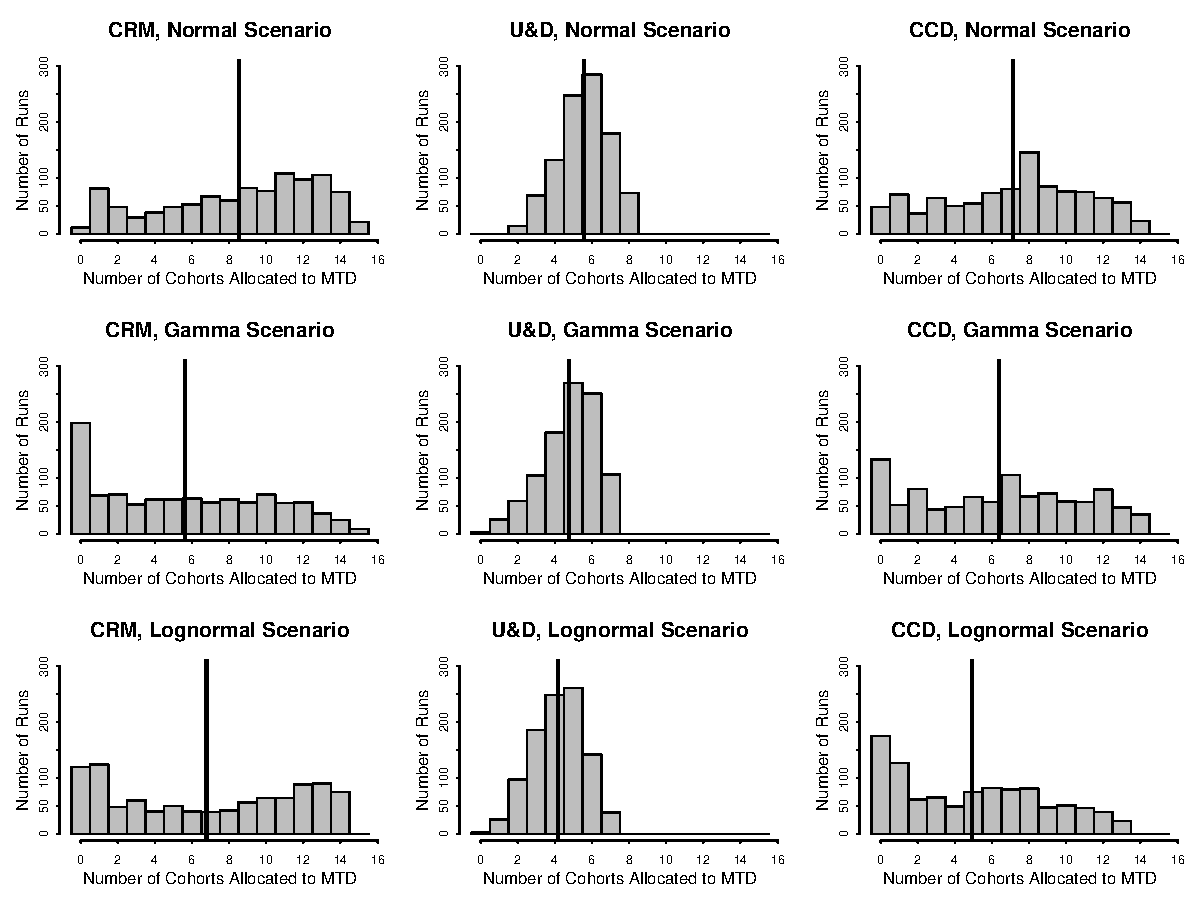
\includegraphics[scale=0.73]{nstar}
\end{center}
\caption{Simulation-ensemble distributions of $n^*$, the number of cohorts assigned the true MTD during the experiment  (excluding the first cohort), under three forms of the dose-toxicity rate function $F$ (top to bottom), and the CRM (left),  UD (center) and CCD (right) designs, as described in the text. Ensemble size was 1000 runs.}\label{fig:nstar}
\end{figure}

With LMP1s, the mean values of $n^*$ (marked by a solid vertical line in each histogram) are indeed larger than with UD designs. With UD designs, $n^*$ values in different runs are tightly clustered around their theoretical expectation. By contrast, LMP1s display far greater variability. With Gamma-distributed toxicity thresholds (middle row), the most common CRM $n^*$ value -- by far -- was \emph{zero} allocations to the true MTD during the entire experiment, except for the opening cohort which was also the true MTD in this case. The nonparametric CCD displays similar behavior to CRM, indicating that this is a universal LMP1 trait, almost unaffected by specific design choice.

The importance of Figure~\ref{fig:nstar}'s message  should not be understated.  Phase~I researchers spend years planning and running a single experiment, and would benefit very little from optimistic reports about high average $n^*$ values, when the underlying individual-experiment distribution is (at best) nearly uniform between zero and $n$. The focus on LMP1's high ensemble-average $n^*$ values has been misguided and misleading. LMP1 designs cannot reliably promise researchers an advantage over UD designs in this respect, because the increase in ensemble-average values comes at the price of greatly increasing the risk of individual experiments with very low $n^*$.

A thorough inspection of the phenomenon illustrated in Figure~\ref{fig:nstar} and its causes are beyond the scope of this chapter, but it can be easily confirmed and reproduced by anyone running a dose-finding simulation study. In any case, contrary to prevalent opinion in many circles, when all aspects are considered UD designs do in fact hold their own compared with the most sophisticated, cutting-edge LMP1s, even in  Phase~I cancer applications to which the latter are tailored. Some hybrid designs attempting to combine the advantages of UD and LMP1 designs, are in development \citep[Ch.~5]{Oron07}.

%%%%%%%%%%%%%%%%%%%%%%%%%%%%%%% SECTION 5 STARTS HERE

\chapter{Summary and Practical Recommendations}\label{sec:summary}

UD procedures constitute a family of simple designs, empowering researchers with limited statistical training to use them independently. However, beneath the simplicity lie the power and elegance of UD's Markov chain behavior, whose fundamentals were explored here. With this additional knowledge, researchers can bolster their experiment's design against the known pitfalls. As this chapter shows, there are still many open challenges, especially with regard to estimation of the target quantile. Researchers are encouraged to consult with a statistician cognizant of modern UD methodology, even when their experiment seems to follow a well-trodden path. When choosing a specific UD design, it should be noted that the scientifically-mandated toxicity target rate $\Gamma$ may not necessarily equal $F^*$, the toxicity frequency of the balance point $x^*$. Certainly this is the case with $k$--in--a--row and GUD, whose $F^*$ values are usually irrational.

The issue of appropriate sample sizes for UD designs is taken very lightly in some fields, where $n\approx 10$ or even less are considered acceptable. One should keep in mind that despite the geometric-rate erasure of initial conditions, UD estimation precision is still largely governed by the same root-$n$ convergence rates of non-sequential estimation \citep[Section~1.2]{Oron07} . Moreover, the available data are a small sample of binary responses scattered over several dose levels (for regression estimators), or a small sample of correlated dose allocations (for averaging estimators). While some experiments might appear very well-behaved, that impression might be misleading unless the underlying variance of toxicity thresholds is far smaller than anticipated. Ultimately, increasing the sample size is the only sure method for substantially reducing estimation error.

In many fields, researchers use the number of reversals  as stopping criterion. \cite{Garc:Pere:Forc:1998} surveyed all experiments determining ``vision thresholds'' published in the 1990s. The most common design used by researchers was the $k$--in--a--row UD design, and most experiments stopped after a fixed number of reversals, typically $6-12$, equivalent to roughly $20-50$ observations. Many environmental toxicity studies also use reversals for stopping, albeit far earlier than in vision research (2-4 reversals using the classical UD design; equivalent to roughly $8-15$ subjects). Due to the properties of reversals outlined above, a reversal-based stopping rule will generally stop earlier precisely for those experiments that would actually most benefit from continuing longer, because their trajectory was more erratic and generated more frequent reversals. Other fields consistently use a fixed sample size. For example, in anesthesiology, $n=30$ seems to be a common choice for classical UD experiments \citep{Capo:Parp:Lyon:Colu:Cell:Mini:2001,Camo:Capo:Lyon:Colu:Epid:2004}. \cite{Pace:styl:tutor:2007} recommend a sample size of $n\geq 20$ for the classical UD design.

Another practical challenge, that should be considered in conjunction with sample size, is choosing the number of dose levels $M$. In order to develop nicely-peaked UD allocation distributions that greatly improve estimation precision and help reduce the extent of excursions (Fig.~\ref{fig:pi}), ideally at least $3-4$ levels are needed on each side of the balance point $x^*$. This translates to at least $8-10$ levels. However, increasing $M$ also increases the number of subjects needed to erase the starting-dose effect -- and there is no guarantee that the experiment will take a beeline from the starting point $x_1$ directly to the vicinity of $x^*$ without a detour on the way (see again Fig.~\ref{fig:traject}).  In essence, this is the well-known bias-variance tradeoff in a somewhat unusual reincarnation.

As to starting dose, when regulatory authorities allow beginning anywhere in $\mathcal{X}$ rather than at its lower boundary, we would recommend a starting dose that minimizes the expected length of this initial tour -- i.e., a level lying midway between the boundaries, in terms of the number of subjects required to reach each boundary under the transition rules. When starting ``in the middle'' is not possible or not advisable, and when sample size is constrained ($n\leq 30$), $M$ will probably need to be smaller, in order to allow the experiment to comfortably reach the top boundary of $\mathcal{X}$ if so needed.

In summary, the most generic sample-size and dose-spacing recommendation we can provide is this: use $M\geq 8$ dose levels and choose $n$ large enough to allow at least half the experiment to meander around the balance point $x^*$, assuming the worst-case distance from the starting point. If this is technically infeasible, decrease $M$.

From \cite{Weth:Sequ:1963} onwards, researchers have examined designs that begin with coarse spacing, which is reduced  gradually as the experiment progresses. This brings UD procedures closer to the paradigm of stochastic approximation \citep{Robb:Monro:Asto:1951}, which allocates gradually decreasing dose increments on a continuous dose scale. However, numerical studies have repeatedly shown little benefit from these elaborate down-scaling schemes; simply put, it is difficult to evade the UD design's bias-variance tradeoff in this manner \citep{Garc:Pere:Forc:1998}. In the same vein, even though UD design's adaptive nature might invite researchers to implement adaptive stopping rules, we  advise against the practice. With an experiment already constrained by low information content (binary observations) and a small sample size, adaptive stopping rules introduce an unnecessary source of additional variability.

When the experiment's goal is dose-selection from $\mathcal{X}$ rather than estimation of $F^{-1}(\Gamma)$ (see Section~\ref{sec:other}), the tradeoff beteen $n$ and $M$ is somewhat different. Here, with too many dose levels the experiment might never provide enough data to tell their toxicity rates apart. A simple rule-of-thumb is that in order to distinguish between the toxicity rates of adjacent doses, $n$ must be large enough, and $M$ small enough, so that for each dose interval around $x^*$ there will be at least $3-4$ subjects, preferably $5$ or more, whose toxicity thresholds fall in the interval.  Thus, with $n=20$ and $\Gamma\approx 0.3$ one should probably design no more than $5-7$ dose levels, and with $n=10$ no more than $M=4$. These rough guidelines assume a starting point in the middle of $\mathcal{X}$. If toxicity concerns dictate a start near the bottom of $\mathcal{X}$, $n$ should be increased by at least the minimal number of subjects required to travel halfway up $\mathcal{X}$ according to the design's rules. To attain the same expected sampling density around the median, the classical UD design can make do with perhaps $20\%-40\%$ fewer subjects than the $\Gamma\approx 0.3$ rules-of-thumb, while using the same $M$. Conversely, very extreme quantiles ($\Gamma\leq 0.1$) would require considerably more subjects.

\chapter{Historical Notes}\label{sec:history}

The most widely-cited ``origin paper'' for the classical UD design is \cite{Dixo:Mood:Amet:1948}. The article was part of an adaptation of a memorandum submitted to the Applied Mathematics Panel by the Statistical Research Group, Princeton University.  The Statistical Research Group operated under a contract with the Office of Statistical Research and Development which was directed by the Applied Mathematics Panel of the National Defense Research Committee.  Their work was motivated by experiments at the Bruceton naval explosive testing site in Pennsylvania during World War II. As often happens in research, Nobel laureate \cite{vonB:anew:1947} came up with a similar design for hearing-threshold determination, almost simultaneously.  An internal Navy report of a lesser known UD design that is more similar to $k$--in--a--row (Ted Anderson, personal communication) predates Dixon and Mood by two years  \citep{Ande:McCa:Tuke:Stai:1946}. While that report is widely cited, we have been unable to locate the original manuscript.

The first study known to have written about UD design's Markov properties is \cite{Derm:Nonp:1957}, the same article that presented the first biased-coin UD design. \cite{Weth:Chen:Vasu:est:1966} introduced the still-hugely-popular reversal estimator a few years later, mostly based on the narrow edge this estimator had over averages of all treatments, in numerical simulations using logistically-distributed thresholds. The time being the early 1960's, Wetherill had to travel across the Atlantic to the US and be awarded precious computer time there, in order to perform the simulations -- a feat that was a main topic in the Royal Statistical Society discussion of the \cite{Weth:Sequ:1963} article. From that point onward, dose-finding research has been wedded -- sometimes blissfully, at other times less so -- to numerical simulation studies.

Other important contributions to UD theory and design in the 1950s and 1960s were made by \cite{BrownleeEtAl53} and \cite{Tsut:asym:1967,Tsut:rand:1967}. Then the methodological UD design trail gradually ran cold, until its relative reawakening in recent decades as described throughout this chapter.
